\documentclass[11pt,a4paper]{article}
\usepackage[margin=2.3cm]{geometry}
\usepackage[T1]{fontenc}
\usepackage[utf8]{inputenc}
\usepackage{lmodern}
\usepackage{amsmath,amssymb,mathtools,bm}
\usepackage{graphicx}
\usepackage{booktabs}
\usepackage{caption}
\captionsetup{font=small,labelfont=bf,margin=0.5cm}
\usepackage{xcolor}
\usepackage{tikz}
\usetikzlibrary{arrows.meta}
\usepackage{microtype}
\usepackage{enumitem}
\setlist{itemsep=2pt,topsep=4pt}
\usepackage[colorlinks=true,linkcolor=blue!45!black,citecolor=blue!45!black,urlcolor=blue!45!black]{hyperref}
\graphicspath{{../results/}}

\newcommand{\ket}[1]{\lvert #1\rangle}
\newcommand{\bra}[1]{\langle #1\rvert}
\newcommand{\braket}[2]{\langle #1\vert #2\rangle}
\newcommand{\ev}[1]{\langle #1\rangle}
\newcommand{\Tr}{\operatorname{Tr}}
\newcommand{\Nex}{\hat N_{\mathrm{exc}}}
\newcommand{\Lio}{\mathcal{L}}
\newcommand{\E}{\mathcal{E}}
\newcommand{\ad}{a^\dagger}
\newcommand{\Zeven}{Z_{\mathrm{even}}}
\newcommand{\Zodd}{Z_{\mathrm{odd}}}

\title{\textbf{Geometric phases as diagnostics of a dissipative time crystal}\\[4pt]
\large The switched open Dicke model: background, construction and first results}
\author{Working report for the GP-for-Discrete-Time-Crystal project}
\date{November 2026}

\begin{document}
\maketitle

\begin{abstract}
\noindent
A discrete time crystal is a periodically driven system whose response repeats only every
\emph{two} (or more) drive periods. Nguyen and Reichman recently asked what happens to such
order in a finite cavity-QED system, the periodically switched open Dicke model, and found
a surprisingly non-monotonic approach to the large-$N$ limit~\cite{nguyen2026}. This report
does three things. First, it introduces time crystals, the model and its two phase
transitions (superradiance and time-crystalline order) from scratch. Second, it recalls the
geometric-phase (GP) diagnostic of our oscillator paper~\cite{sun_gp}, in which winding a
drive phase generates a closed loop of steady states. Third, it shows how that diagnostic
carries over. The main results are:
\begin{itemize}[leftmargin=1.2em]
\item The construction extends \emph{exactly} to the Dicke model. Winding the phase of the
  counter-rotating coupling is generated by the excitation number $\Nex=\ad a+J_z+N/2$ and
  reduces to a single-state formula, just as the squeezing phase does in the Kerr resonator.
\item That GP reproduces, in the Dicke model, the weak-drive and phase-transition behaviour of
  the oscillator paper. It switches sharply from $0$ to $\pi$ across the superradiant
  transition, exactly where the branch-mixing Liouvillian gap closes.
\item The time crystal needs one more ingredient: the GP of the physical one-period loop of the
  Floquet steady state. In the ordered limit it is quantized to $\pi$ when the drive swaps the
  two symmetry-broken branches and to $0$ when it does not. It thus reads the sign of the
  leading parity-odd Floquet eigenvalue.
\item Exact Floquet numerics reproduce the non-monotonic size dependence of the time-crystal
  lifetime. The GP describes the \emph{structure} of the finite-$N$ state, but does not by
  itself predict that size dependence.
\end{itemize}
\end{abstract}

\setcounter{tocdepth}{1}
\tableofcontents
\clearpage

%=========================================================================================
\section{Time crystals from scratch}\label{sec:tc}
%=========================================================================================

\subsection{Breaking time-translation symmetry}

An ordinary crystal breaks a symmetry of its own laws. The Hamiltonian is unchanged by any
translation $x\to x+a$, yet the atoms sit on a lattice that is unchanged only by the discrete
lattice translations. In 2012 Wilczek asked whether \emph{time} translation could be broken in
the same way~\cite{wilczek2012}. For systems in thermal equilibrium the answer is no: no-go
theorems rule out a ground state or Gibbs state whose observables oscillate in
time~\cite{bruno2013,watanabe2015}.

The question becomes meaningful for periodically driven (Floquet) systems,
\begin{equation}
H(t+T)=H(t).
\end{equation}
Such a system has a \emph{discrete} time-translation symmetry, $t\to t+T$. The natural
response repeats with the drive period $T$. A \emph{discrete time crystal} (DTC) is a system
whose observables instead repeat only every $nT$ with $n\ge2$. For period doubling, measuring
once per period (``stroboscopically'') gives
\begin{equation}
\ev{O(mT)} \simeq (-1)^m A,\qquad m=0,1,2,\dots
\label{eq:subharmonic}
\end{equation}
Equation~\eqref{eq:subharmonic} alone is not enough. A single spin flipped by a $\pi$ pulse
every period also alternates. The defining property is \emph{rigidity}. If the pulse angle is
imperfect, $\pi(1-\epsilon)$, a lone spin drifts away from \eqref{eq:subharmonic} at a rate
$\propto\epsilon$. A time crystal instead stays locked to period $2T$ over a finite range of
$\epsilon$, because interactions or dissipation correct the error, and the locking survives
longer and longer as the system grows. Three requirements are usually listed:
\begin{enumerate}[label=(\roman*)]
\item a subharmonic response;
\item rigidity against perturbations of the drive;
\item persistence, i.e.\ a lifetime that diverges with system size.
\end{enumerate}

The main obstacle is heating. An interacting closed system absorbs energy from the drive and
ends at infinite temperature, where nothing oscillates. Proposed remedies are disorder (many-body
localization), slow heating (pre-thermalization), and \emph{dissipation}: coupling to a bath that
removes the absorbed energy~\cite{khemani2016,else2016,sacha2018}. DTCs have been observed with
trapped ions~\cite{zhang2017}, spins in diamond~\cite{choi2017}, and as a \emph{dissipative} time
crystal in an atom--cavity system~\cite{kessler2021}. The model in this report is of this last,
dissipative type~\cite{gong2018}.

\subsection{Floquet language: one-period map, lifetime and phase transition}\label{sec:floquet}

For an open system described by a Lindblad master equation $\dot\rho=\Lio(t)[\rho]$, evolving
for one period defines a linear map on density matrices,
\begin{equation}
\rho\big((m+1)T\big)=\E\big[\rho(mT)\big],\qquad
\E[r_\alpha]=\mu_\alpha r_\alpha,\quad |\mu_\alpha|\le1 .
\end{equation}
$\E$ is a completely positive, trace-preserving map. Its eigenvalue $\mu_0=1$ belongs to the
\emph{Floquet steady state} $\rho_F$, the state the system settles into after many periods. All
other eigenvalues have $|\mu_\alpha|\le1$. Expanding the initial state in the eigenmodes gives
\begin{equation}
\rho(mT)=\rho_F+\sum_{\alpha\ge1}c_\alpha\,\mu_\alpha^{\,m}\,r_\alpha .
\label{eq:floquet_expansion}
\end{equation}
Period doubling requires an eigenvalue close to $-1$. Then $\mu^m\approx(-1)^m$ produces
\eqref{eq:subharmonic}. Three consequences organise everything that follows.
\begin{itemize}
\item \textbf{Finite systems cannot be time crystals forever.} For finite $N$ the steady state
  is generically unique and every other $|\mu_\alpha|<1$. The alternation therefore decays, with
  lifetime
  \begin{equation}
  \tau_{\rm DTC}=-\frac{T}{\ln|\mu_1|},
  \end{equation}
  where $\mu_1$ is the eigenvalue closest to $-1$.
\item \textbf{The time-crystal \emph{phase} is a limit.} A genuine DTC phase means
  $\mu_1\to-1$ as $N\to\infty$: the spectral gap of $\E$ closes at ``quasi-energy'' $\pi$. This
  is the Floquet analogue of the Liouvillian gap closing that signals a dissipative phase
  transition~\cite{minganti2018}.
\item \textbf{The order is hidden in $\rho_F$.} If the dynamics has a symmetry that the time
  crystal breaks (here a $\mathbb Z_2$ parity), the unique $\rho_F$ must be symmetric. Every
  symmetry-breaking expectation value vanishes in it, even when the system is a near-perfect
  time crystal. Section~\ref{sec:model} shows this explicitly.
\end{itemize}

%=========================================================================================
\section{The model and its phase transitions}\label{sec:model}
%=========================================================================================

\subsection{The switched open Dicke model}

Nguyen and Reichman~\cite{nguyen2026}, following Gong, Hamazaki and Ueda~\cite{gong2018},
consider $N$ two-level atoms coupled to one lossy cavity mode:
\begin{equation}
H(t)=\omega_c\,\ad a+\omega J_z+\frac{2\lambda(t)}{\sqrt N}\,(a+\ad)\,J_x,
\qquad
\lambda(t)=\begin{cases}\lambda_0,& 0\le t \bmod T<T/2,\\ 0,& T/2\le t\bmod T<T,\end{cases}
\label{eq:H}
\end{equation}
\begin{equation}
\dot\rho=-i[H(t),\rho]+\kappa\Big(a\rho\ad-\tfrac12\{\ad a,\rho\}\Big).
\label{eq:lindblad}
\end{equation}
Here $J_\alpha=\tfrac12\sum_i\sigma^{(i)}_\alpha$ are collective spin operators. The coupling
is switched on for the first half of each period and off for the second; $T=2\pi$. The
frequencies are $\omega_c=1-\epsilon$ and $\omega=1+\epsilon$, so the detuning is
$\epsilon=(\omega-\omega_c)/2$. Throughout, $\kappa=0.05$ and $\lambda_0=1$, and the system
starts with an empty cavity and all spins along $+x$. Both $H$ and the loss act collectively, so
the dynamics stays in the symmetric sector $j=N/2$, of dimension $N+1$. This makes exact
numerics possible for small $N$.

\paragraph{Symmetry.} The parity operator
\begin{equation}
\Pi=e^{\,i\pi(\ad a+J_z+N/2)}:\qquad a\to-a,\quad J_{x,y}\to-J_{x,y},\quad J_z\to J_z
\end{equation}
commutes with $H(t)$ at all times, and $D[-a]=D[a]$. The master equation therefore commutes with
the superoperator $\mathcal P(\rho)=\Pi\rho\Pi$. Every Liouvillian and Floquet eigenmode is
either parity-even or parity-odd. Order parameters such as $\ev{a}$ and $\ev{J_x}$ are odd.

\subsection{First phase transition: superradiance}\label{sec:superradiance}

Keep the coupling on, $\lambda(t)=\lambda$, and treat the large-$N$ limit in mean field. Write
$\alpha=\ev a$ and $\bm s=\ev{\bm J}/j$. The cavity follows the spin,
\begin{equation}
\dot\alpha=-(i\omega_c+\tfrac\kappa2)\alpha-i\frac{2\lambda}{\sqrt N}\ev{J_x}
\quad\Rightarrow\quad
\alpha_{\rm ss}=-\frac{2\lambda}{\sqrt N}\,\frac{\ev{J_x}}{\omega_c-i\kappa/2},
\end{equation}
and the spin precesses about an effective field
$\bm B=\big(\tfrac{4\lambda}{\sqrt N}\mathrm{Re}\,\alpha,\;0,\;\omega\big)$. A stationary spin
must lie along $\bm B$. Inserting $\alpha_{\rm ss}$ gives either the normal state
$s_x=0,\ s_z=-1$, or a second solution
\begin{equation}
s_z=-\Big(\frac{\lambda_c}{\lambda}\Big)^2,\qquad
s_x=\pm\sqrt{1-\Big(\frac{\lambda_c}{\lambda}\Big)^4},\qquad
\lambda_c=\frac12\sqrt{\frac{\omega}{\omega_c}\Big(\omega_c^2+\frac{\kappa^2}4\Big)},
\label{eq:lambda_c}
\end{equation}
which exists only for $\lambda>\lambda_c\approx0.50$. In this \emph{superradiant} phase the cavity
holds a macroscopic field,
\begin{equation}
\frac{|\alpha|^2}{N}=\frac{\lambda^2}{\omega_c^2+\kappa^2/4}\Big[1-\Big(\frac{\lambda_c}{\lambda}\Big)^4\Big],
\label{eq:photons}
\end{equation}
which gives $0.956$ at $\lambda=1$; the exact value at $N=6$ is $0.950$. The two solutions
$\pm$ are mapped into each other by $\Pi$. This is spontaneous breaking of the $\mathbb Z_2$
symmetry, and the transition is continuous (second order).

\paragraph{What a dissipative phase transition looks like at finite $N$.} The steady state of a
Lindblad equation is a nonequilibrium object, and a dissipative phase transition is a
non-analytic change of it as a parameter crosses a critical value, in the limit
$N\to\infty$~\cite{minganti2018,kirton2019}. At finite $N$ the steady state is unique and
parity-symmetric: $\ev{a}=0$ exactly, even deep in the superradiant phase. The symmetry breaking
shows up instead in the Liouvillian spectrum. The steady state becomes an incoherent mixture of
the two branches, and the slowest parity-odd eigenvalue (the rate at which the branches mix)
goes to zero as $N\to\infty$ for $\lambda>\lambda_c$. We will see this rate collapse by orders of
magnitude across $\lambda_c$ already at $N=6$ (Fig.~\ref{fig:superradiant}c).

\subsection{Second phase transition: from superradiance to a time crystal}\label{sec:dtc_mechanism}

Now switch the coupling on and off. The free half period ($\lambda=0$, loss aside) applies
\begin{equation}
U_{\rm off}=e^{-i\pi(\omega_c\ad a+\omega J_z)}
\;\overset{\epsilon=0}{=}\;e^{-i\pi(\ad a+J_z)}\;\propto\;\Pi ,
\label{eq:Uoff}
\end{equation}
because $a\to e^{-i\pi}a=-a$ and $J_\pm\to-J_\pm$. \emph{The free segment is the parity
operation}: it maps the superradiant branch with $(+\alpha,+s_x)$ onto the one with
$(-\alpha,-s_x)$. The coupled segment, which includes the cavity loss, pulls the state towards
the nearest branch. One period therefore maps branch $A$ to branch $B$ and back, and
\begin{equation}
\ev{\sigma_x(mT)}\propto(-1)^m .
\end{equation}
For $\epsilon\ne0$ the free rotation is imperfect,
$U_{\rm off}\propto\Pi\,e^{\,i\pi\epsilon(\ad a-J_z)}$, and dissipation corrects the error;
this is the rigidity of Sec.~\ref{sec:tc}. In mean field the ordered region is mapped by the
Floquet multipliers of the linearized one-period map. It is stable for $\mu_{\rm MF}\approx-1$
and becomes chaotic for $|\mu_{\rm MF}|>1$ at large detuning~\cite{nguyen2026}.

Figure~\ref{fig:intro} shows the exact dynamics for $N=4$. The magnetization alternates
(panel~b). The cavity's phase-space distribution has two lobes at $\pm\alpha$, and the dominant
lobe changes side every period (panels~c,~d). The Floquet steady state, panel~e, contains both
lobes with equal weight. It has $\ev{\sigma_x}=0$, yet it is made of two branches that the drive
keeps exchanging. This is the hidden order of Sec.~\ref{sec:floquet}, and reading it is the
central task for a geometric diagnostic.

\begin{figure}[t]
\centering
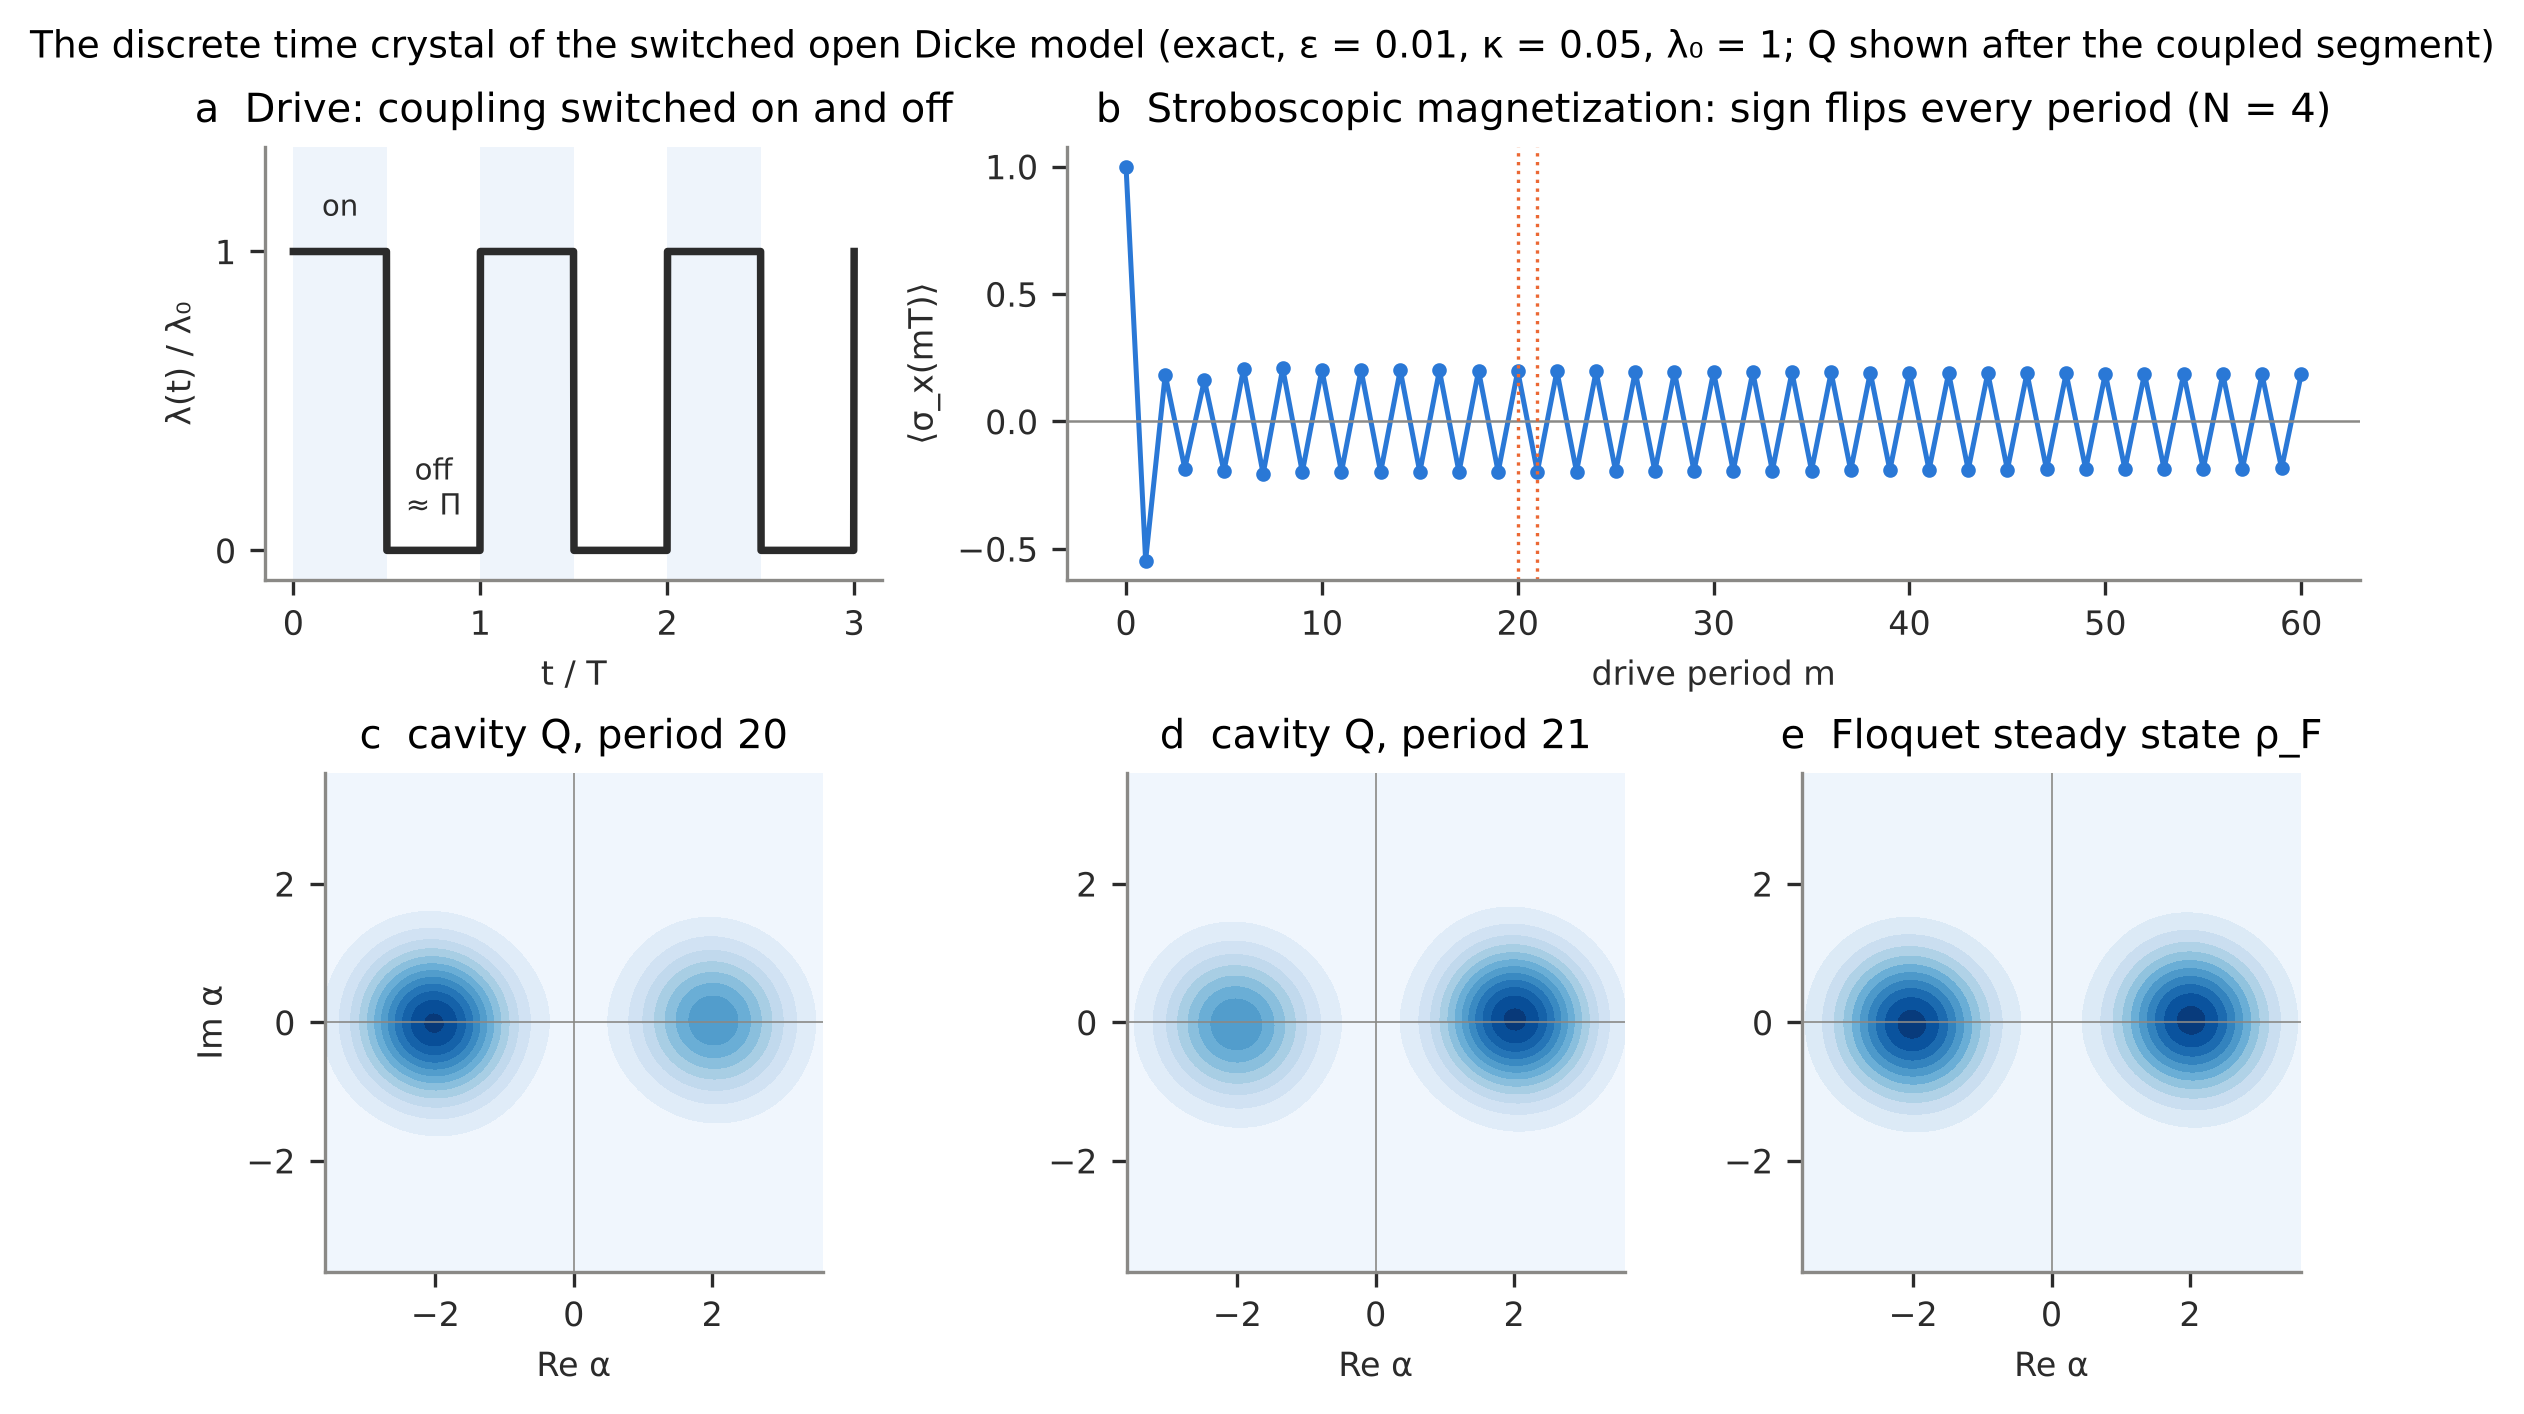
\includegraphics[width=\linewidth]{report_dtc_intro.png}
\caption{The dissipative time crystal of the switched open Dicke model (exact, $N=4$,
$\epsilon=0.01$, $\kappa=0.05$, $\lambda_0=1$).
(a)~Drive protocol; the free half period acts approximately as the parity $\Pi$.
(b)~Stroboscopic magnetization, alternating in sign every period.
(c,d)~Husimi function of the cavity after the coupled segment in periods 20 and 21: the dominant
lobe changes side.
(e)~The Floquet steady state $\rho_F$ holds both lobes equally, so all order parameters vanish
in it.}
\label{fig:intro}
\end{figure}

\subsection{What happens at finite size}\label{sec:finiteN}

Gong \emph{et al.} predicted that the lifetime of this time crystal grows monotonically with
$N$~\cite{gong2018}. Nguyen and Reichman tested this with three methods: exact Lindblad
evolution for $N\le10$, quantum trajectories for $N\le20$, and a stochastic truncated Wigner
approximation (TWA) for large $N$. Cumulant expansions fail because a Gaussian closure cannot
represent two branches at once. Their findings~\cite{nguyen2026}:
\begin{itemize}
\item \textbf{Three regimes} of $\ev{\sigma_x(mT)}$: \emph{unstable} (no order, or order below
  $0.05$); \emph{transient} (decay over hundreds of periods); and \emph{pre-thermal} (no visible
  decay over the simulated time, near $\epsilon\approx0$).
\item \textbf{Non-monotonic size dependence.} In the transient window
  ($\epsilon\in[0.05,0.11]$) there is an island of \emph{faster} decay at intermediate sizes,
  $N<20$, instead of a steady slowing with $N$. In the pre-thermal window the amplitude drops
  below $0.05$ at $N\sim100$–$500$ before recovering.
\item \textbf{Mechanism.} The mean-field dynamics has two period-2 attractors, in phase and out
  of phase with the mean-field orbit, separated by an intricate basin boundary. The initial
  quantum uncertainty, of width $\propto1/\sqrt N$, straddles both basins, so the amplitude is
  roughly $(f_{\rm in}-f_{\rm out})A_{\rm MF}$. In the transient regime, chaotic decorrelation of
  trajectories adds to the decay.
\end{itemize}
In the language of Sec.~\ref{sec:floquet}, all of this concerns \emph{how} $\mu_1$ approaches
$-1$ as $N$ grows. Two phase transitions are therefore in play. The superradiant one creates
two branches. The time-crystalline one makes the drive exchange them indefinitely, with
$\mu_1\to-1$.

%=========================================================================================
\section{The geometric phase as a diagnostic}\label{sec:gp}
%=========================================================================================

\subsection{Kinematic geometric phase of a loop of states}

For a path of density matrices $t\mapsto\rho(t)$, $0\le t\le\tau$, with spectral decomposition
$\rho(t)=\sum_k\lambda_k(t)\ket{\psi_k(t)}\bra{\psi_k(t)}$, the kinematic mixed-state geometric
phase is~\cite{tong2004}
\begin{equation}
\Gamma=\arg Z,\qquad
Z=\sum_k\sqrt{\lambda_k(0)\lambda_k(\tau)}\,\braket{\psi_k(0)}{\psi_k(\tau)}\,
\exp\!\Big(-\!\int_0^\tau\braket{\psi_k}{\dot\psi_k}\,dt\Big).
\label{eq:tong}
\end{equation}
It is gauge invariant and defined for any path, unitary or not. The modulus $|Z|$ (the
``visibility'') measures cancellation between the phasors of different eigenvectors.
Degenerate eigenvalues are handled by parallel transport within each eigenspace~\cite{singh2003}.

\subsection{Loops from winding a drive phase}

The key idea of our oscillator paper~\cite{sun_gp} is a \emph{physical} loop. Winding the phase
of a drive generates a closed family of steady states. If the Liouvillian is covariant,
$\Lio_\varphi[R\rho R^\dagger]=R\,\Lio_0[\rho]\,R^\dagger$ with $R(\varphi)=e^{-i\varphi Q}$ and
$Q$ an operator with integer spectrum, then $\rho_{\rm ss}(\varphi)=R\,\rho_{\rm ss}R^\dagger$.
The eigenvalues stay fixed, the eigenvectors are $R\ket{\psi_k}$, and
$\braket{\psi_k}{\partial_\varphi\psi_k}=-i\ev{Q}_k$. Equation~\eqref{eq:tong} then reduces to
a \emph{single-state formula},
\begin{equation}
Z=\sum_k\lambda_k\,e^{2\pi i\ev{Q}_k}\quad(\varphi:0\to2\pi),\qquad
Z_{\rm half}=\sum_k\lambda_k\,\pi_k\,e^{i\pi\ev{Q}_k}\quad(\varphi:0\to\pi,\ R(\pi)=\Pi).
\label{eq:single_state}
\end{equation}
The half loop closes whenever $R(\pi)$ is a symmetry of the state. It then carries the parity
$\pi_k=\pm1$ of each eigenvector as an endpoint factor; this is Eq.~(S14) of~\cite{sun_gp}.
For the harmonically driven oscillator $Q=\hat n$. For the two-photon-driven Kerr resonator the
squeezing phase $\theta$ winds with $\varphi=\theta/2$, so $\theta:0\to2\pi$ is the half loop.
The paper showed that this GP is the quadratic imprint of drive-induced coherences at weak drive
(the synchronization regime), and that it reorganizes at critical points and dissipative phase
transitions.

\subsection{Parity sectors and the ideal two-branch limit}\label{sec:lemma}

Both models here have a $\mathbb Z_2$ parity. When every state along a loop commutes with $\Pi$,
its eigenvectors can be chosen with definite parity, and the amplitude splits exactly:
\begin{equation}
Z=\Zeven+\Zodd,\qquad
\Delta\equiv\arg\big(\Zeven\,\Zodd^{\,*}\big),\qquad
C\equiv\frac{-2\,\mathrm{Re}(\Zeven\Zodd^{\,*})}{|\Zeven|^2+|\Zodd|^2}\in[-1,1].
\label{eq:sectors}
\end{equation}
$\Delta$ is the relative geometric phase of the two sectors. $C$ is a weight-aware version that
equals $1$ only for $\Zodd=-\Zeven$. One lemma organizes everything that follows.

\medskip\noindent\textbf{Lemma (ideal two-branch state).}
Suppose that along the loop
\begin{equation}
\rho(t)=\tfrac12\big[\rho_A(t)+\Pi\rho_A(t)\Pi\big],
\qquad \rho_A(t)=\sum_k p_k\ket{a_k(t)}\bra{a_k(t)},
\end{equation}
where branch $A$ and its parity image $B$ have orthogonal supports and are not connected by the
motion, $\braket{\Pi a_k}{\partial_t a_k}=0$. Then:
\begin{itemize}
\item if the loop \emph{exchanges} the branches, $\ket{a_k(\tau)}=e^{i\beta_k}\Pi\ket{a_k(0)}$,
  then $\Zodd=-\Zeven$, so $\Delta=\pi$ and $Z=0$;
\item if the loop \emph{returns} each branch to itself, then $\Zodd=\Zeven$ and $\Delta=0$.
\end{itemize}

\noindent\emph{Proof.} The eigenvectors of $\rho$ come in pairs
$\ket{e_k}=(\ket{a_k}+\Pi\ket{a_k})/\sqrt2$ and $\ket{o_k}=(\ket{a_k}-\Pi\ket{a_k})/\sqrt2$, each
of weight $p_k/2$. The assumptions give
$\braket{e_k}{\partial_t e_k}=\braket{o_k}{\partial_t o_k}=\braket{a_k}{\partial_t a_k}$, so both
members of a pair acquire the same transport phase. In the exchanging case
$\ket{e_k(\tau)}=e^{i\beta_k}\ket{e_k(0)}$ while $\ket{o_k(\tau)}=-e^{i\beta_k}\ket{o_k(0)}$. The odd
member gets an extra $-1$ and the even member does not. In the returning case neither does.
$\square$

\medskip
The relative phase is therefore a $\mathbb Z_2$ \emph{holonomy}: in the ideal limit it is $\pi$
or $0$, depending on whether the loop swaps the two branches, as on a Möbius band. Overlap
between the branches, and tunnelling between them during the loop, move $\Delta$ away from the
quantized value. These are finite-size effects.

\subsection{What a GP diagnostic of the time crystal must do}

Section~\ref{sec:model} sets three requirements:
\begin{enumerate}[label=(\roman*)]
\item the loop should be \emph{physical}, generated by winding something an experiment controls;
\item ideally it should reduce to a single state, as in Eq.~\eqref{eq:single_state};
\item it must see what the magnetization cannot, namely the hidden two-branch structure of the
  symmetric $\rho_F$, and whether the drive swaps the branches.
\end{enumerate}
Figure~\ref{fig:loops} previews the two loops that meet these requirements. Before them comes
the construction we tried first, and the reason it fails.

\begin{figure}[t]
\centering
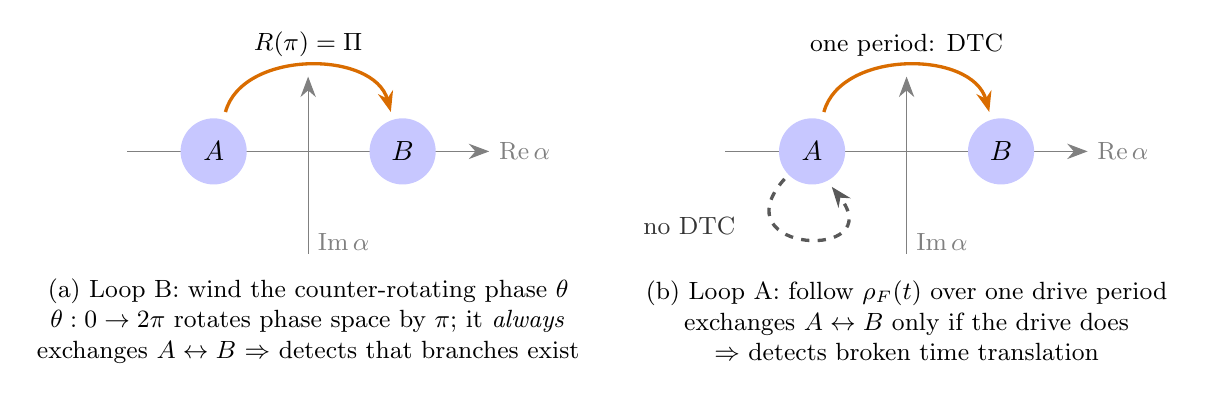
\begin{tikzpicture}[scale=1.0,>={Stealth[length=2.6mm]}]
\begin{scope}
  \draw[->,gray] (-2.3,0)--(2.3,0) node[right]{\small $\mathrm{Re}\,\alpha$};
  \draw[->,gray] (0,-1.3)--(0,0.95);
  \node[gray,right,font=\small] at (0,-1.15) {$\mathrm{Im}\,\alpha$};
  \fill[blue!22] (-1.2,0) circle (0.42); \node at (-1.2,0) {$A$};
  \fill[blue!22] (1.2,0) circle (0.42); \node at (1.2,0) {$B$};
  \draw[->,very thick,orange!85!black] (-1.05,0.5) to[out=75,in=105] node[midway,above=1pt,fill=white,inner sep=1.5pt,text=black]{\small $R(\pi)=\Pi$} (1.05,0.5);
  \node[align=center,font=\small] at (0,-2.15) {(a) Loop B: wind the counter-rotating phase $\theta$\\
  $\theta:0\to2\pi$ rotates phase space by $\pi$; it \emph{always}\\ exchanges $A\leftrightarrow B$ $\Rightarrow$ detects that branches exist};
\end{scope}
\begin{scope}[xshift=7.6cm]
  \draw[->,gray] (-2.3,0)--(2.3,0) node[right]{\small $\mathrm{Re}\,\alpha$};
  \draw[->,gray] (0,-1.3)--(0,0.95);
  \node[gray,right,font=\small] at (0,-1.15) {$\mathrm{Im}\,\alpha$};
  \fill[blue!22] (-1.2,0) circle (0.42); \node at (-1.2,0) {$A$};
  \fill[blue!22] (1.2,0) circle (0.42); \node at (1.2,0) {$B$};
  \draw[->,very thick,orange!85!black] (-1.05,0.5) to[out=75,in=105] node[midway,above=1pt,fill=white,inner sep=1.5pt,text=black]{\small one period: DTC} (1.05,0.5);
  \draw[->,very thick,dashed,gray!70!black] (-1.55,-0.35) .. controls (-2.4,-1.3) and (-0.2,-1.4) .. (-0.95,-0.45);
  \node[font=\small,gray!40!black,anchor=east] at (-2.05,-0.95) {no DTC};
  \node[align=center,font=\small] at (0,-2.15) {(b) Loop A: follow $\rho_F(t)$ over one drive period\\
  exchanges $A\leftrightarrow B$ only if the drive does\\ $\Rightarrow$ detects broken time translation};
\end{scope}
\end{tikzpicture}
\caption{The two loops used in this report, drawn in the cavity phase space of
Fig.~\ref{fig:intro}e. By the Lemma of Sec.~\ref{sec:lemma}, a loop that exchanges the two
branches gives a relative sector phase $\Delta=\pi$, and one that returns them gives $\Delta=0$.}
\label{fig:loops}
\end{figure}

%=========================================================================================
\section{A first attempt, and why it fails}\label{sec:fail}
%=========================================================================================

The first construction in this project kept the single-state formula~\eqref{eq:single_state}
but replaced $\hat n$ by a fixed spin generator,
$Q_{xy}=j+uJ_x+\sqrt{1-u^2}J_y$ with $u=1/(4N)$, and evaluated it on $\rho(mT)$ after each
period. $\hat n$ itself is useless here: it commutes with $\Pi$, so its GP cannot tell the two
branches apart. $Q_{xy}$ satisfies $\Pi Q_{xy}\Pi=N-Q_{xy}$, which implies
$Z_Q[\Pi\rho\Pi]=Z_Q[\rho]^*$. Hence $\mathrm{Im}\,Z_Q$ is parity-odd and alternates in a time
crystal.

The trouble is that \emph{every} parity-odd functional $F$ (magnetization, $\mathrm{Im}\,Z_Q$, or
anything else) carries the same late-time information. Insert the expansion
\eqref{eq:floquet_expansion} and use two facts. First, $F[\rho_F]=0$, since $\rho_F$ is
symmetric. Second, the linear response of $F$ to a parity-even perturbation vanishes by
symmetry. Therefore
\begin{equation}
F\big[\rho(mT)\big]=c_1\,\mu_1^{\,m}\;DF[\rho_F](r_1)\;+\;\text{(faster-decaying terms)} .
\label{eq:odd_functional}
\end{equation}
All parity-odd signals decay at the \emph{same} rate $-\ln|\mu_1|$ and differ only by a constant
prefactor.

We checked this by computing $\mu_1$ directly, with Arnoldi iteration on the one-period map
restricted to the parity-odd sector (Fig.~\ref{fig:late}). At $\epsilon=0.01$, $N=2$, the
Floquet rate is $-\ln|\mu_1|=0.008462$ per period. Fits over periods 500–700 give $0.008462$
(magnetization), $0.008457$ (transverse GP) and $0.008448$ (paired GP). The late-time ratios of
the GP signals to the magnetization settle to constants, $1.390$ and $1.573$. At
$\epsilon=-0.056$ the Floquet rate is $0.043301$, and fits over periods 150–200 give $0.04330$,
$0.04330$ and $0.04329$. The negative ratio $-0.473$ explains the sign flip seen in the project's
earlier trace figures.

There is one nuance. Because $\rho_F$ has nearly degenerate even/odd eigenvalue pairs,
$\mathrm{Im}\,Z_Q$ stays nonlinear in the odd component for a long time. The GP signals reach
the asymptotic rate only after about 400 periods, and a fit over a short window is \emph{biased}
(by $5$–$19\%$ between periods 100 and 300). Finally, $Z_Q$ is identically real in $\rho_F$.

\emph{Lesson:} a GP evaluated on the decaying odd component is just another order parameter. A
useful diagnostic must (i) come from a physical loop and (ii) read the structure of $\rho_F$
itself.

\begin{figure}[t]
\centering
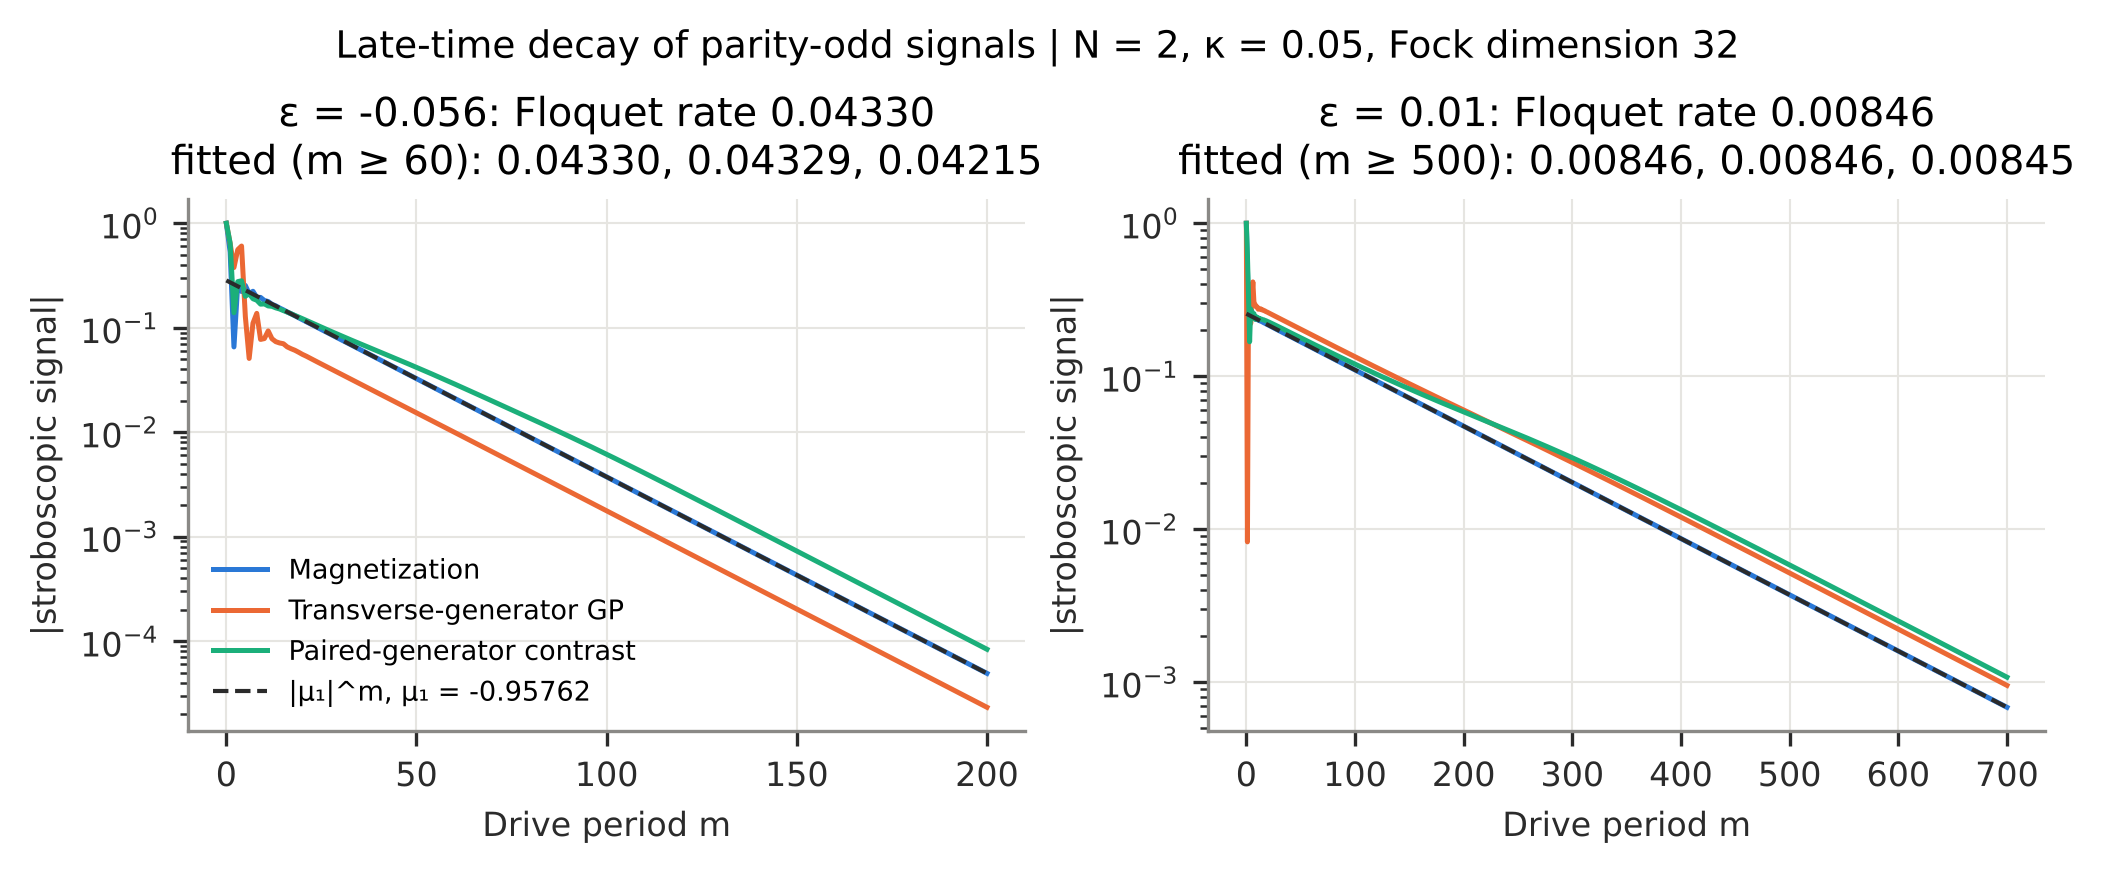
\includegraphics[width=0.92\linewidth]{floquet_gp_late_time.png}
\caption{Why the stroboscopic fixed-generator GP is not new information. Magnetization (blue),
transverse-generator GP (orange) and paired-generator GP (green) all decay as $|\mu_1|^m$
(dashed), where $\mu_1$ is computed independently from the Floquet spectrum ($N=2$, Fock
dimension 32).}
\label{fig:late}
\end{figure}

%=========================================================================================
\section{An exact extension: winding the counter-rotating phase}\label{sec:loopB}
%=========================================================================================

\subsection{The covariance and the single-state formula}

The missing ingredient is the right generator. Split the Dicke coupling into its co-rotating
part (which conserves excitations) and its counter-rotating part (which creates or destroys
them in pairs), and give the latter a phase $\theta$:
\begin{equation}
H_\theta(t)=\omega_c\ad a+\omega J_z+\frac{\lambda(t)}{\sqrt N}
\Big[\underbrace{(aJ_++\ad J_-)}_{\text{co-rotating}}
+\underbrace{(e^{i\theta}aJ_-+e^{-i\theta}\ad J_+)}_{\text{counter-rotating}}\Big].
\label{eq:Htheta}
\end{equation}
At $\theta=0$ this is Eq.~\eqref{eq:H}, since $J_++J_-=2J_x$. Let
\begin{equation}
\Nex=\ad a+J_z+\tfrac N2,\qquad R(\varphi)=e^{-i\varphi\Nex}.
\end{equation}
$\Nex$ counts photons plus atomic excitations and has integer spectrum. Since
$RaR^\dagger=e^{i\varphi}a$ and $RJ_-R^\dagger=e^{i\varphi}J_-$, the co-rotating terms are
invariant while the counter-rotating terms acquire $e^{\pm2i\varphi}$:
\begin{equation}
R(\varphi)\,H_\theta(t)\,R^\dagger(\varphi)=H_{\theta+2\varphi}(t),
\qquad D[e^{i\varphi}a]=D[a].
\label{eq:covariance}
\end{equation}
The Liouvillian is covariant at every time $t$. Steady states and Floquet steady states
therefore obey $\rho_\theta=R(\theta/2)\,\rho_0\,R^\dagger(\theta/2)$. This is precisely the
structure of the Kerr resonator, with $\hat n\to\Nex$ and the squeezing phase replaced by
$\theta$. In both cases a term that changes the conserved number by $\pm2$ breaks U(1) down to
the parity $\Pi=e^{i\pi\Nex}$. Equation~\eqref{eq:single_state} applies directly:
\begin{equation}
\theta:0\to4\pi:\ \ Z_{\rm full}=\sum_k\lambda_k e^{2\pi i\ev{\Nex}_k},
\qquad
\theta:0\to2\pi:\ \ Z_{\rm half}=\sum_k\lambda_k\pi_k e^{i\pi\ev{\Nex}_k}=\Zeven+\Zodd,
\label{eq:loopB}
\end{equation}
and we write $\Delta_B$ for the relative sector phase of the half loop.

\paragraph{Checks and realization.} Numerically, $\theta=0$ reproduces the original Liouvillian
to $10^{-15}$. The steady state at $\theta=1.3$ equals the rotated one to $10^{-10}$, and
Eq.~\eqref{eq:loopB} equals the kinematic GP of the explicitly tracked orbit to $10^{-5}$. In
cavity-assisted Raman realizations of the Dicke model, the co- and counter-rotating couplings
come from separate Raman channels~\cite{dimer2007}. $\theta$ is then a relative laser phase, so
winding it is a genuine drive-phase winding, as in the oscillator paper. Such platforms also
avoid the $A^2$ term that would otherwise remove the transition.

\paragraph{What loop B measures.} The half loop ends with $R(\pi)=\Pi$, which exchanges the two
superradiant branches of \emph{any} parity-symmetric state. By the Lemma, $\Delta_B\to\pi$
whenever two well-separated branches exist. For coherent-state branches the result is the Kerr
cat formula of~\cite{sun_gp}: the even and odd members of a pair differ in $\ev{\Nex}$ by an
amount exponentially small in the branch separation, and
$|\Delta_B|=\pi[1-2N_B/\sinh 2N_B]$ for branches with $N_B$ excitations. Loop B is therefore a
geometric order parameter for the $\mathbb Z_2$ breaking (Fig.~\ref{fig:loops}a).

\subsection{Weak coupling: the GP as the imprint of pair coherences}

In the normal phase the counter-rotating terms create coherences between $\Nex$ sectors that
differ by $2$, much as a weak two-photon drive creates $\rho_{n,n+2}$. Split
$\rho=\rho_0+\delta\rho$, with $\rho_0$ block-diagonal in $\Nex$, eigenvectors $\ket k$ and
weights $p_k$. To first order the eigenvalues are unchanged and the eigenvectors mix,
$\ket{k'}=\ket k+\sum_l\frac{\bra l\delta\rho\ket k}{p_k-p_l}\ket l$. Since $\ev{\Nex}$ is an
integer in $\rho_0$, only its second-order shift enters, and summing over pairs gives
\begin{equation}
\Gamma_{\rm full}\simeq2\pi\sum_{v<w}(w-v)\sum_{k\in v,\;l\in w}
\frac{\big|\bra k\delta\rho\ket l\big|^2}{p_k-p_l} .
\label{eq:weak}
\end{equation}
This is the oscillator paper's weak-drive result with $\hat n\to\Nex$. Table~\ref{tab:weak}
compares it with the exact GP. The GP is quadratic in the coupling and nearly independent of
$N$ at weak coupling, and the formula breaks down towards $\lambda_c$, just as the
synchronization formula breaks down towards the Hopf threshold.

\begin{table}[h]
\centering
\begin{tabular}{@{}lcccccc@{}}
\toprule
$\lambda$ & 0.05 & 0.10 & 0.20 & 0.30 & 0.40 & 0.45 \\
\midrule
exact $\Gamma_{\rm full}/\pi$, $N=2$ & 0.00252 & 0.01025 & 0.04424 & 0.11309 & 0.24070 & 0.33911 \\
Eq.~\eqref{eq:weak} / exact, $N=2$ & 1.001 & 1.004 & 1.016 & 1.043 & 1.085 & 1.150 \\
Eq.~\eqref{eq:weak} / exact, $N=4$ & 1.001 & 1.005 & 1.020 & 1.055 & 1.140 & 1.145 \\
\bottomrule
\end{tabular}
\caption{Weak-coupling GP of loop B in the undriven model ($\kappa=0.05$, $\epsilon=0.01$)
against the perturbative formula~\eqref{eq:weak}.}
\label{tab:weak}
\end{table}

\subsection{The superradiant transition seen by the GP}

Figure~\ref{fig:superradiant} shows loop B across the superradiant transition of the undriven
model for $N=2,4,6$. Exact steady states have residuals $\le10^{-13}$ and top-three Fock
populations $\le3\times10^{-5}$.
\begin{itemize}
\item \textbf{A sharp switch.} The photon number per atom rises smoothly (panel~a), but
  $|\Delta_B|$ switches from $\approx0$ to $\pi$ (panel~b). The switch sharpens and moves
  towards the mean-field $\lambda_c=0.500$ as $N$ grows: $|\Delta_B|=\pi/2$ at
  $\lambda\approx0.87$, $0.73$ and $0.68$ for $N=2,4,6$. At $N=6$ it jumps from $0.25\pi$ to
  $0.95\pi$ between $\lambda=0.65$ and $0.80$.
\item \textbf{It follows the spectral signature.} The switch coincides with the collapse of the
  slowest parity-odd Liouvillian rate, the rate at which the two branches mix (panel~c). At
  $N=6$ that rate falls from $4\times10^{-2}$ at $\lambda=0.65$ to $5\times10^{-3}$ at $0.70$ and
  $5\times10^{-4}$ at $0.80$. The single-state GP tracks the finite-size precursor of the
  dissipative phase transition.
\item \textbf{Phasor cancellation.} The full-loop visibility $|Z_{\rm full}|$ (panel~d) has a
  minimum exactly at the crossover: $0.23$, $0.21$ and $0.44$ for $N=2,4,6$. This is the
  interference mechanism of the oscillator paper. The half-loop visibility (panel~f) goes to zero
  because $\Zodd\to-\Zeven$.
\end{itemize}

\begin{figure}[t]
\centering
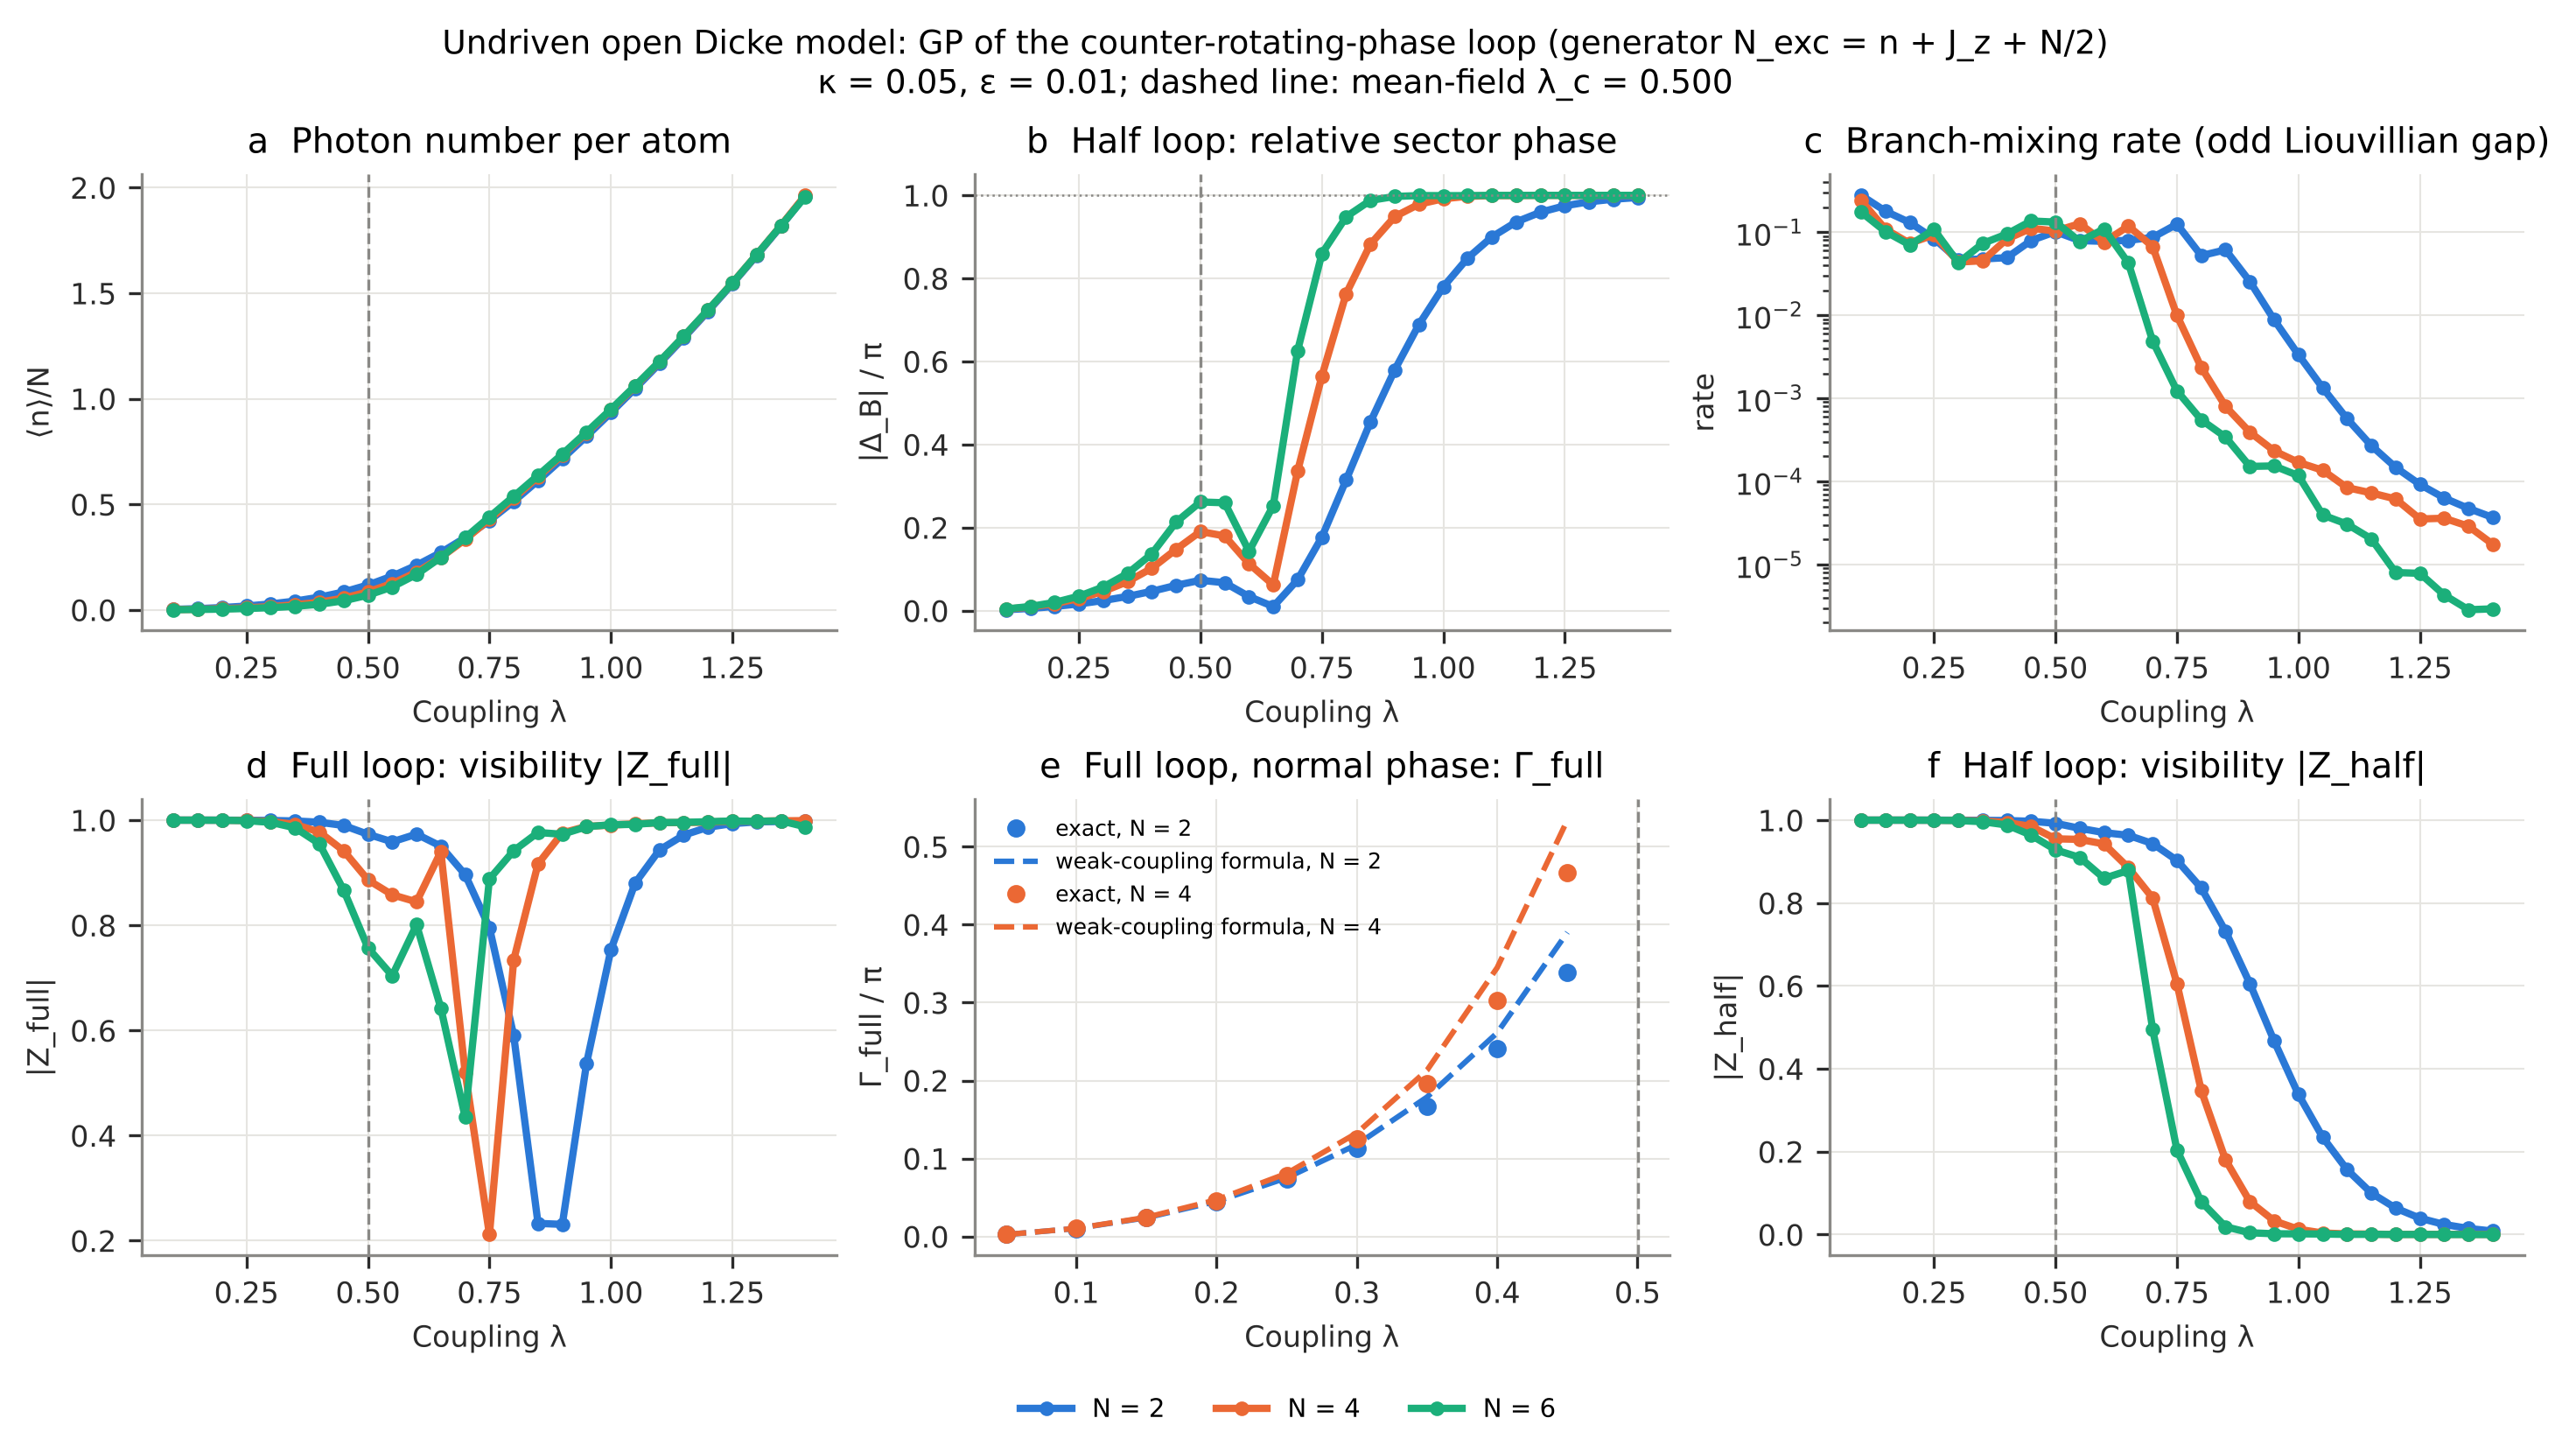
\includegraphics[width=\linewidth]{extension_superradiant.png}
\caption{Loop B across the superradiant transition of the undriven open Dicke model.
(a)~Photon number per atom. (b)~Relative sector phase of the half loop.
(c)~Slowest parity-odd Liouvillian rate (branch mixing). (d)~Full-loop visibility.
(e)~Weak-coupling GP: exact (dots) against Eq.~\eqref{eq:weak} (dashed). (f)~Half-loop
visibility. Dashed vertical line: mean-field $\lambda_c$, Eq.~\eqref{eq:lambda_c}.}
\label{fig:superradiant}
\end{figure}

Loop B thus reproduces, in the Dicke model, the oscillator paper's weak-drive regime and its
phase-transition signatures. It cannot, however, tell a time crystal from mere superradiance.
Its half loop exchanges the branches \emph{by construction}, whether or not the drive does. That
requires a second, genuinely dynamical loop.

%=========================================================================================
\section{The time crystal: the geometric phase of one drive period}\label{sec:loopA}
%=========================================================================================

\subsection{The micromotion loop}

The Floquet steady state is periodic, $\rho_F(t+T)=\rho_F(t)$, so following it through one
period traces a \emph{closed loop} of density matrices. Equivalently, $\rho_F(\tau)$ is the
Floquet steady state of the drive shifted in time by $\tau$. Winding the drive's \emph{temporal}
phase $\tau$ over one period therefore generates a closed loop of nonequilibrium steady states.
This is the time-domain counterpart of winding a drive phase. Call it loop A, and let $\Delta_A$
be its relative sector phase. Because $\Pi$ commutes with the dynamics at all times, $\rho_F(t)$
is parity-symmetric along the whole loop, and the sector split~\eqref{eq:sectors} is exact.

Unlike loop B, loop A is not a unitary orbit: the eigenvalues of $\rho_F(t)$ change during the
period. So there is no single-state reduction, and Eq.~\eqref{eq:tong} must be evaluated along
the loop. We propagate $\rho_F$ through the period, diagonalize it in each parity block, follow
each eigenvector by maximum overlap, and accumulate the discrete parallel-transport product.

\paragraph{Prediction.} In a time crystal one period exchanges the branches
(Sec.~\ref{sec:dtc_mechanism}), so the Lemma gives $\Delta_A\to\pi$. If the branches exist but
each returns to itself after a period, $\Delta_A\to0$. Loop A therefore reads whether the drive
swaps the branches, i.e.\ whether time translation is broken (Fig.~\ref{fig:loops}b).

\paragraph{The link to the Kerr half loop.} In the lab frame the two-photon-driven Kerr resonator
is itself period-doubled: its field oscillates at half the pump frequency. Its lab-frame steady
state is $\rho_{\rm lab}(t)=R(\omega t)\,\rho_{\rm ss}\,R^\dagger(\omega t)$ with
$R=e^{-i\varphi\hat n}$. One pump period, $\omega t:0\to\pi$, is exactly the half number rotation.
The half loop of Eq.~\eqref{eq:single_state} is therefore the micromotion GP of a continuously
driven period-doubling oscillator. For the Kerr model loops A and B coincide because its
micromotion is unitary; in the Dicke model they differ.

\subsection{Results}

Figure~\ref{fig:scans} collects loop A for the Dicke model, and Fig.~\ref{fig:phasors} shows the
sector amplitudes themselves. Doubling the time resolution changes $\Delta_A$ by less than
$5\times10^{-4}$\,rad, and Fock dimensions 24 and 32 agree to $10^{-7}$.

\begin{itemize}
\item \textbf{Coupling} ($N=2$, $\epsilon=0.01$; Fig.~\ref{fig:scans}a,e). Without period
  doubling ($\lambda_0\le0.7$, $\mu_1$ complex) the sectors are in phase,
  $|\Delta_A|\le0.08\pi$ and $|Z_T|\ge0.94$. Once $\mu_1$ becomes real and negative,
  $|\Delta_A|/\pi$ rises through $0.62$, $0.80$, $0.964$ and $0.997$ at
  $\lambda_0=0.9,1.0,1.2,1.4$, while $|Z_T|$ falls to $0.004$.
\item \textbf{Atom number} ($\epsilon=0.01$; Fig.~\ref{fig:scans}d,h). $|\Delta_A|/\pi=0.37$ (at
  $N=1$, no DTC), then $0.80$, $0.972$, $0.990$, $0.995$ and $0.995$ for $N=2$–$6$. The deficit
  $\pi-|\Delta_A|$ falls about twentyfold from $N=2$ to $N=4$.
\item \textbf{The ideal pair, realized.} At $N=4$, $\epsilon=0$ a single eigenvector pair carries
  $98.7\%$ of the weight, with weights $0.4939$ and $0.4929$ and relative holonomy $0.993\pi$.
  This is almost exactly the Lemma.
\item \textbf{Kerr resonator} (Fig.~\ref{fig:kerr}). Resolved by parity, the half loop gives
  $|\Delta|=0.98$–$0.9999\pi$ throughout the bright, period-doubled phase, and $0.05$–$0.13\pi$
  on the vacuum-like side. At $\Delta/|U|=0$ the exact value $0.982\pi$ compares with the
  ideal-cat value $0.989\pi$.
\end{itemize}

\begin{figure}[p]
\centering
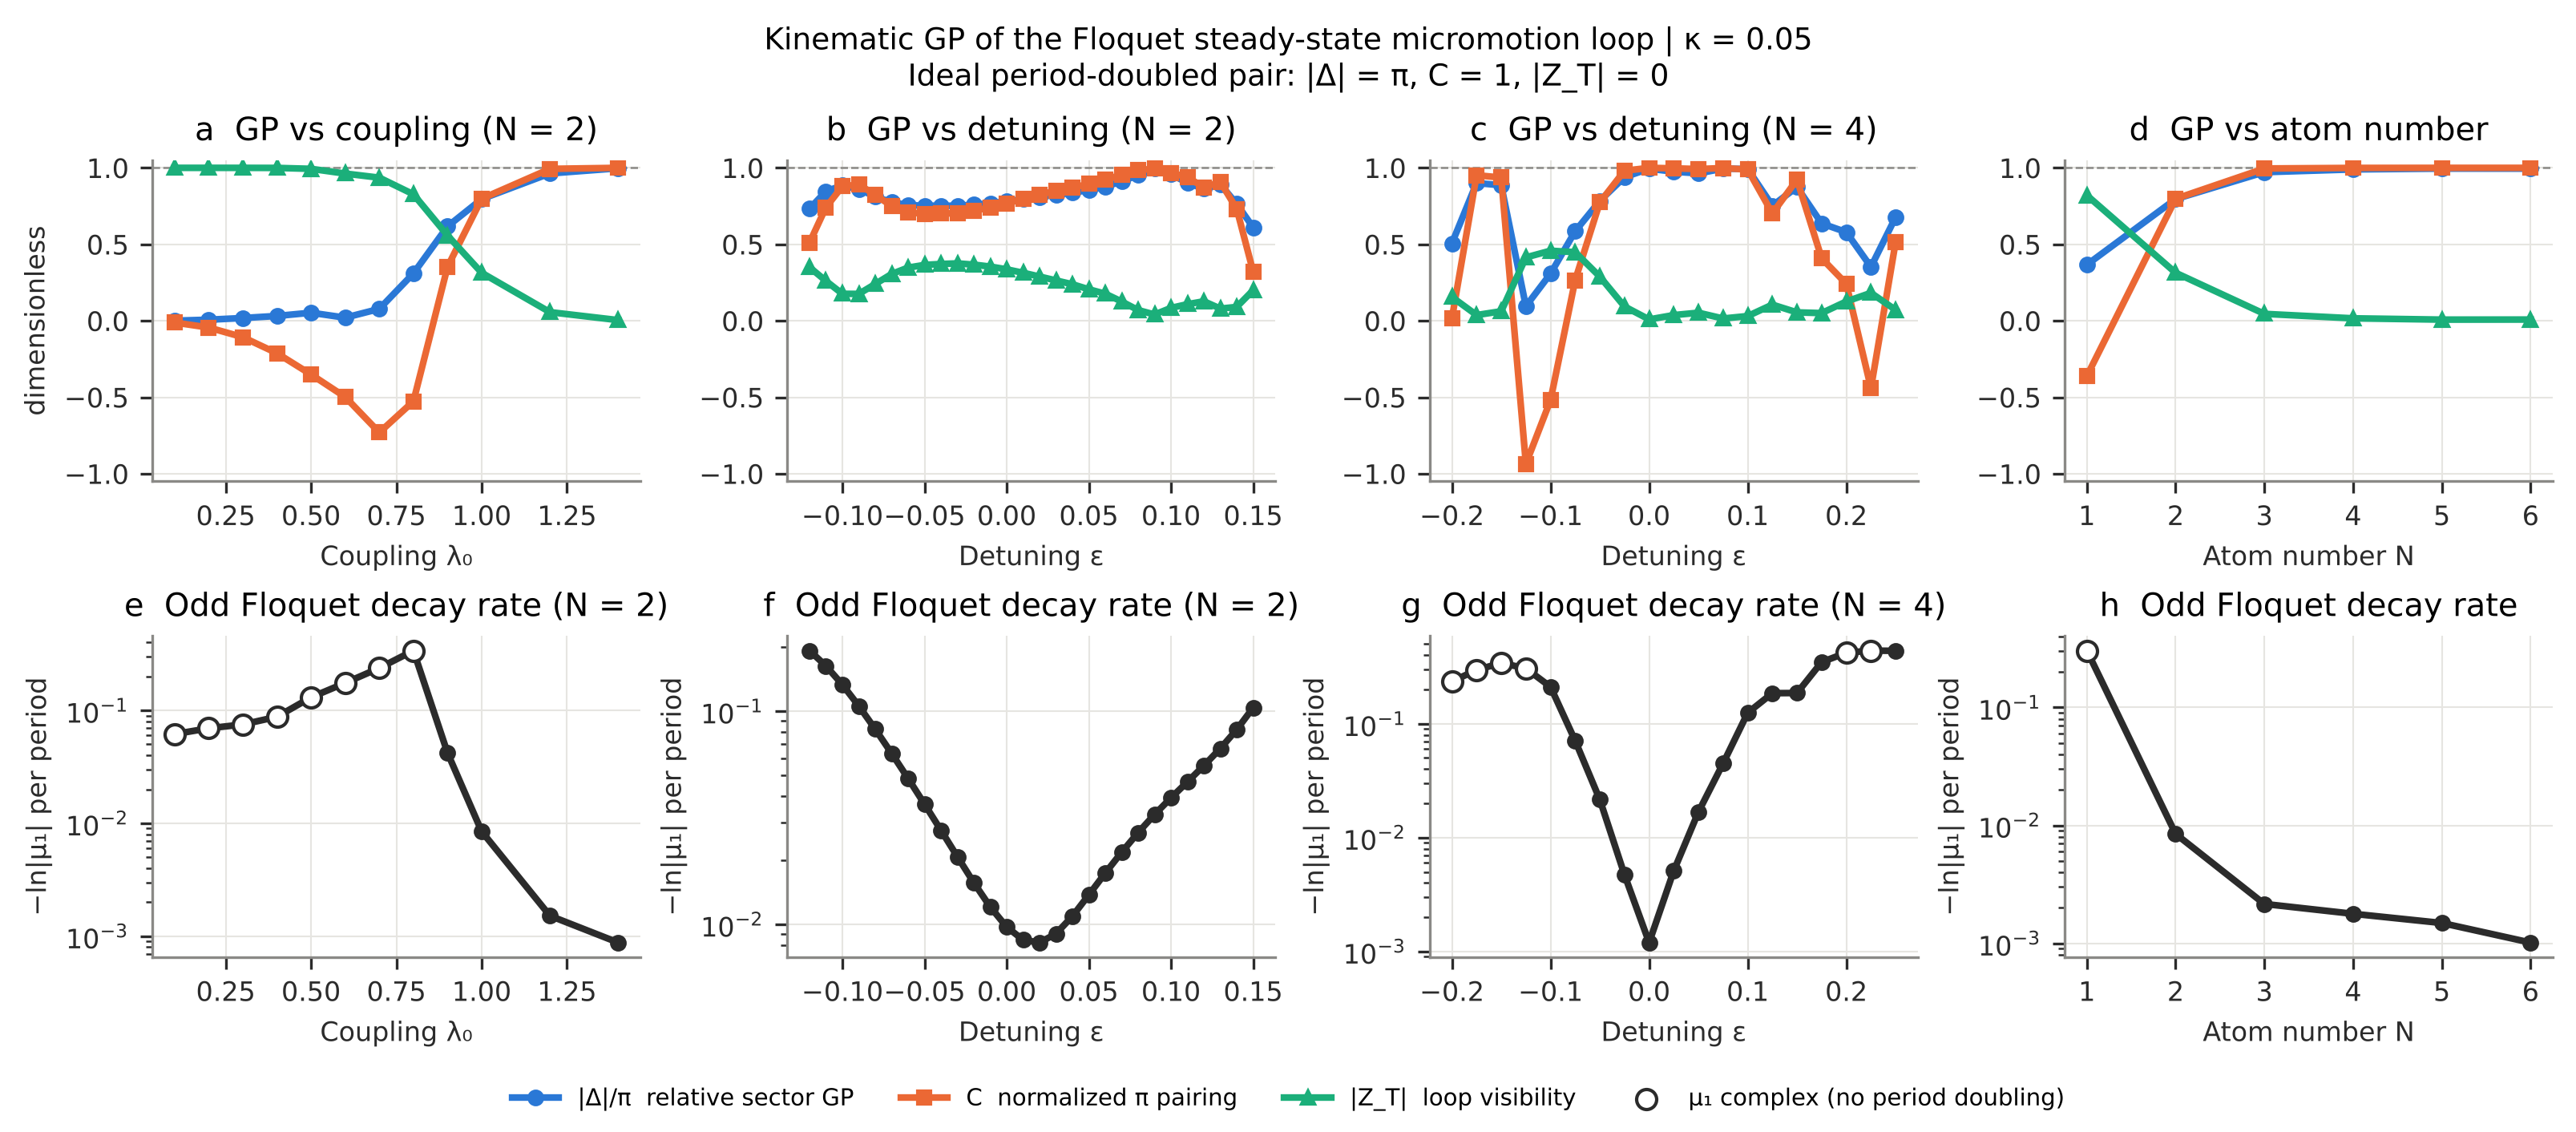
\includegraphics[width=\linewidth]{floquet_gp.png}
\caption{Loop A, the GP of the Floquet steady state over one drive period ($\kappa=0.05$). Top
row: relative sector phase $|\Delta_A|/\pi$ (blue), pairing $C$ (orange) and visibility $|Z_T|$
(green). Bottom row: decay rate $-\ln|\mu_1|$ of the time-crystal mode; open circles mark complex
$\mu_1$ (no period doubling). Columns: coupling scan ($N=2$), detuning scans ($N=2$ and $N=4$),
atom-number scan.}
\label{fig:scans}
\vspace{1.2em}
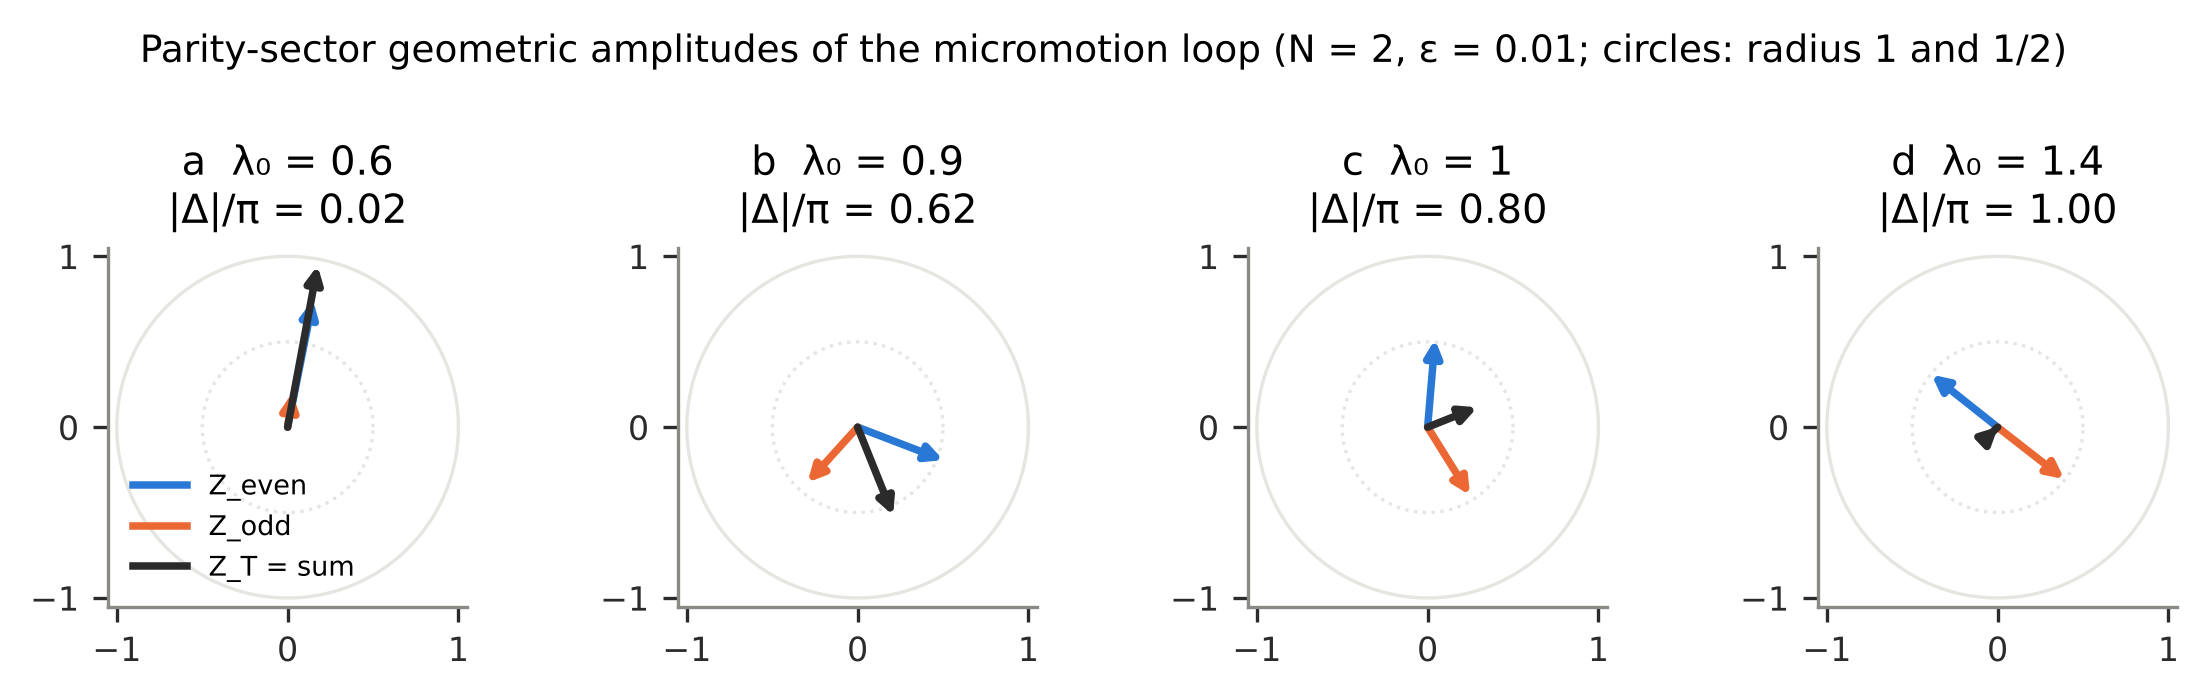
\includegraphics[width=\linewidth]{floquet_gp_phasors.png}
\caption{Sector amplitudes of loop A in the complex plane ($N=2$, $\epsilon=0.01$). As period
doubling sets in, $\Zeven$ and $\Zodd$ rotate from parallel to antiparallel and their sum $Z_T$
vanishes.}
\label{fig:phasors}
\vspace{1.2em}
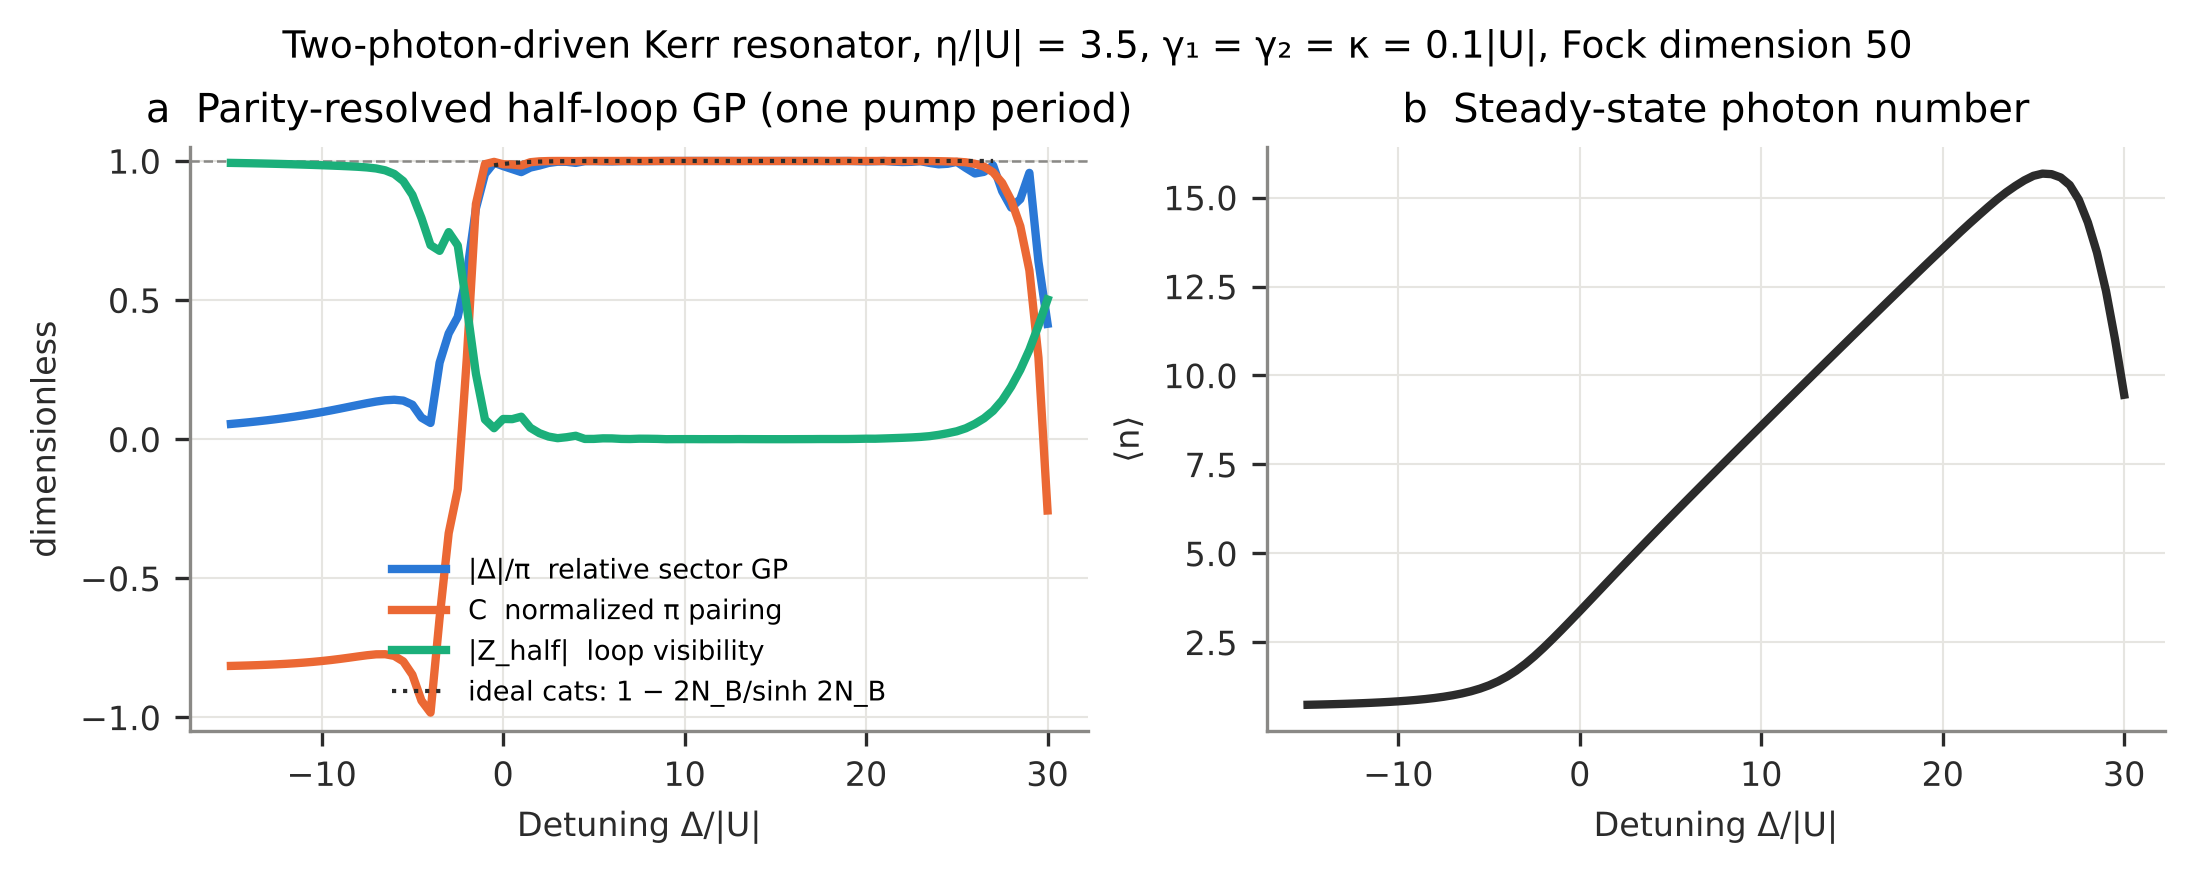
\includegraphics[width=0.95\linewidth]{floquet_gp_kerr.png}
\caption{The Kerr half loop of~\cite{sun_gp}, resolved by parity ($\eta/|U|=3.5$,
$\gamma_1=\gamma_2=\kappa=0.1|U|$, Fock dimension 50). The relative sector phase is $\approx\pi$
throughout the bright (period-doubled) phase. Dotted: ideal-cat formula.}
\label{fig:kerr}
\end{figure}

\paragraph{The detuning scans.} Over the whole $N=2$ window ($-0.12\le\epsilon\le0.15$) $\mu_1$
is real and negative, and $|\Delta_A|$ stays between $0.61\pi$ and $\pi$. It reaches $\pi$ at
$\epsilon\approx0.09$, where the decay is four times faster than at the optimum $\epsilon\approx0.02$.
$\Delta_A$ therefore measures how cleanly the branches are separated and exchanged, not how fast
they mix.

At $N=4$ (Fig.~\ref{fig:scans}c,g), $\Delta_A$ falls together with the time crystal on the
negative side: $0.78\pi$, $0.59\pi$, $0.31\pi$ at $\epsilon=-0.05,-0.075,-0.1$. At two points
outside the time crystal ($\epsilon=-0.15,-0.175$, complex $\mu_1$) the sum-level $|\Delta_A|$ is
accidentally near $0.9\pi$, but there the sector amplitudes have collapsed
($|Z_s|\approx0.12$–$0.18$ against weights $\approx0.5$). A pair-by-pair check removes most of
this ambiguity (Sec.~\ref{sec:finite}).

\subsection{Which loop sees what: a control experiment}

To confirm that loop A detects broken time translation, and not just the existence of branches,
we lengthen the free segment from $\pi$ to $2\pi$. By Eq.~\eqref{eq:Uoff} the free evolution then
approximates $\Pi^2=1$: the branches still form during the coupled segment, but each returns to
itself. Table~\ref{tab:control} and Fig.~\ref{fig:control} show the result.

\begin{table}[h]
\centering
\begin{tabular}{@{}c ccc ccc@{}}
\toprule
& \multicolumn{3}{c}{$T_{\rm off}=\pi$ (branches swapped)} & \multicolumn{3}{c}{$T_{\rm off}=2\pi$ (branches kept)}\\
\cmidrule(lr){2-4}\cmidrule(l){5-7}
$\lambda_0$ & $\mu_1$ & $|\Delta_A|/\pi$ & $|\Delta_B|/\pi$ & $\mu_1$ & $|\Delta_A|/\pi$ & $|\Delta_B|/\pi$\\
\midrule
0.4 & $0.37+0.84i$ & 0.03 & 0.04 & $-0.36-0.81i$ & 0.05 & 0.04\\
0.8 & $-0.70+0.13i$ & 0.31 & 0.27 & $+0.811$ & 0.67 & 0.22\\
1.0 & $-0.9916$ & 0.80 & 0.78 & $+0.9888$ & 0.37 & 0.78\\
1.2 & $-0.9985$ & 0.964 & 0.956 & $+0.9953$ & 0.064 & 0.958\\
1.4 & $-0.9991$ & \textbf{0.997} & 0.995 & $+0.9970$ & \textbf{0.004} & 0.996\\
\bottomrule
\end{tabular}
\caption{Control experiment ($N=2$, $\epsilon=0.01$, $\kappa=0.05$). $\Delta_B$ is evaluated on
$\rho_F$ at the end of the coupled segment.}
\label{tab:control}
\end{table}

Both drives create two branches, so $|\Delta_B|\to\pi$ in both. Only the drive that swaps them
gives $|\Delta_A|\to\pi$; the other gives $|\Delta_A|\to0$, with $\mu_1\to+1$. In the ordered
limit,
\begin{equation}
e^{i\Delta_A}\;\longrightarrow\;\operatorname{sgn}\mu_1 .
\end{equation}
The micromotion GP reads the sign of the leading parity-odd Floquet eigenvalue, i.e.\ whether the
time crystal exists. A time crystal requires \emph{both} $|\Delta_B|\to\pi$ (branches exist) and
$|\Delta_A|\to\pi$ (the drive swaps them).

\begin{figure}[t]
\centering
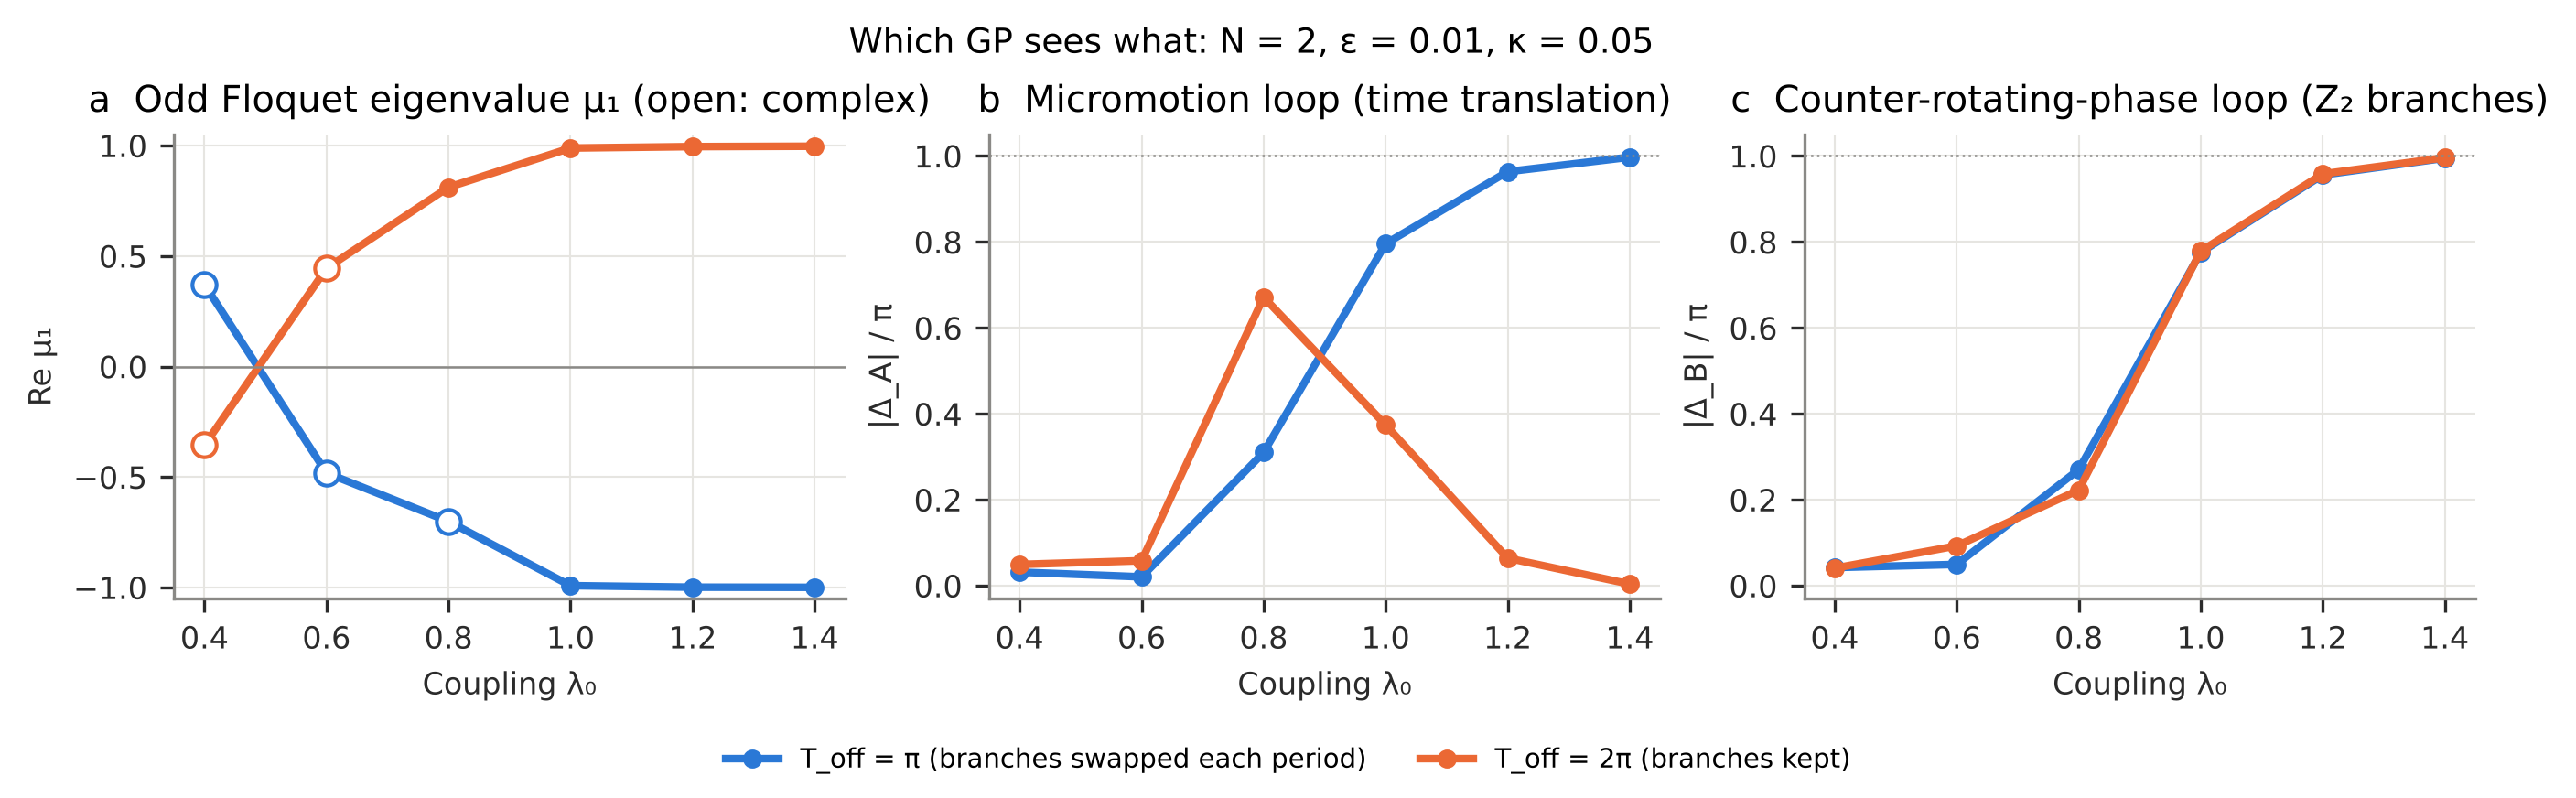
\includegraphics[width=\linewidth]{extension_dtc_control.png}
\caption{Which GP sees what. (a)~Leading parity-odd Floquet eigenvalue; open symbols are complex.
(b)~Loop A follows the sign of $\mu_1$. (c)~Loop B detects the branches in both cases.}
\label{fig:control}
\end{figure}

\subsection{Finite size and the regimes of Nguyen and Reichman}\label{sec:finite}

Finally, return to the finite-size questions of Sec.~\ref{sec:finiteN} (Fig.~\ref{fig:finite}).

\paragraph{The exact spectrum reproduces the non-monotonic size dependence.} In the transient
window ($\epsilon=0.09$) the decay rate per period is
\begin{center}
\begin{tabular}{@{}lcccccc@{}}
\toprule
$N$ & 1 & 2 & 3 & 4 & 5 & 6\\
\midrule
$-\ln|\mu_1|$, $\epsilon=0.09$ & 0.115 & 0.033 & 0.055 & 0.084 & 0.111 & 0.091\\
$-\ln|\mu_1|$, $\epsilon=0.01$ & 0.303$^{*}$ & 0.0085 & 0.0022 & 0.0018 & 0.0015 & 0.0010\\
\bottomrule
\end{tabular}

{\footnotesize $^{*}$complex $\mu_1$: no period doubling.}
\end{center}
It falls, rises and falls again, matching the exact-method ``island'' of Nguyen and Reichman.
Here it follows directly from the Floquet spectrum rather than from fits to trajectories. At
$\epsilon=0.01$ the rate decreases monotonically, as in their pre-thermal window.

\paragraph{What the GP says.} At $\epsilon=0.09$, $|\Delta_A|/\pi=0.55$, $0.999$, $0.85$, $0.88$,
$0.97$, $0.98$ for $N=1$–$6$. The branches stay geometrically swapped while the decay rate rises,
so the non-monotonic decay is not a loss of branch exchange. This is consistent with mixing
between well-defined branches, i.e.\ with the decorrelation mechanism of Nguyen and Reichman.

A second GP quantity is informative here: the \emph{sector coherence}
\begin{equation}
S=\frac{|\Zeven|+|\Zodd|}{w_{\rm even}+w_{\rm odd}},
\end{equation}
where $w$ are the sector weights. $S=1$ when all eigenvectors of a sector acquire the same
micromotion holonomy, and $S$ is small when their holonomies are spread.
\begin{itemize}
\item Along detuning at fixed $N$, $S$ tracks the lifetime: the Spearman correlation between $S$
  and $\ln(-\ln|\mu_1|)$ is $-0.80$ at $N=2$ and $-0.95$ at $N=4$.
\item At $N=4$, $S$ orders the three regimes: $S\ge0.84$ in the pre-thermal window, $0.41$–$0.74$
  in the transient window, and $\le0.42$ beyond it.
\item $S$ does \emph{not} predict the size dependence: at $\epsilon=0.09$ its correlation with the
  rate across $N$ is $+0.03$.
\end{itemize}

\paragraph{A pair-resolved check.} The Lemma predicts more than $\Delta=\pi$: matched even and odd
eigenvectors should have equal weights and holonomies differing by $\pi$. A weight-ranked pair
score
\[
P_{\rm pair}=\frac{\sum_k\min(\lambda_k^e,\lambda_k^o)\,\big[-\cos(\gamma_k^e-\gamma_k^o)\big]}{\sum_k\tfrac12(\lambda_k^e+\lambda_k^o)}
\]
gives $0.987$ at the $N=4$ optimum, but $-0.04$ at $\epsilon=-0.15$. There the sum-level
$\Delta_A$ was accidentally $0.89\pi$. At $\epsilon=-0.175$ a residual $+0.35$ remains, so the
pair-resolved quantity is the one to report.

\begin{figure}[t]
\centering
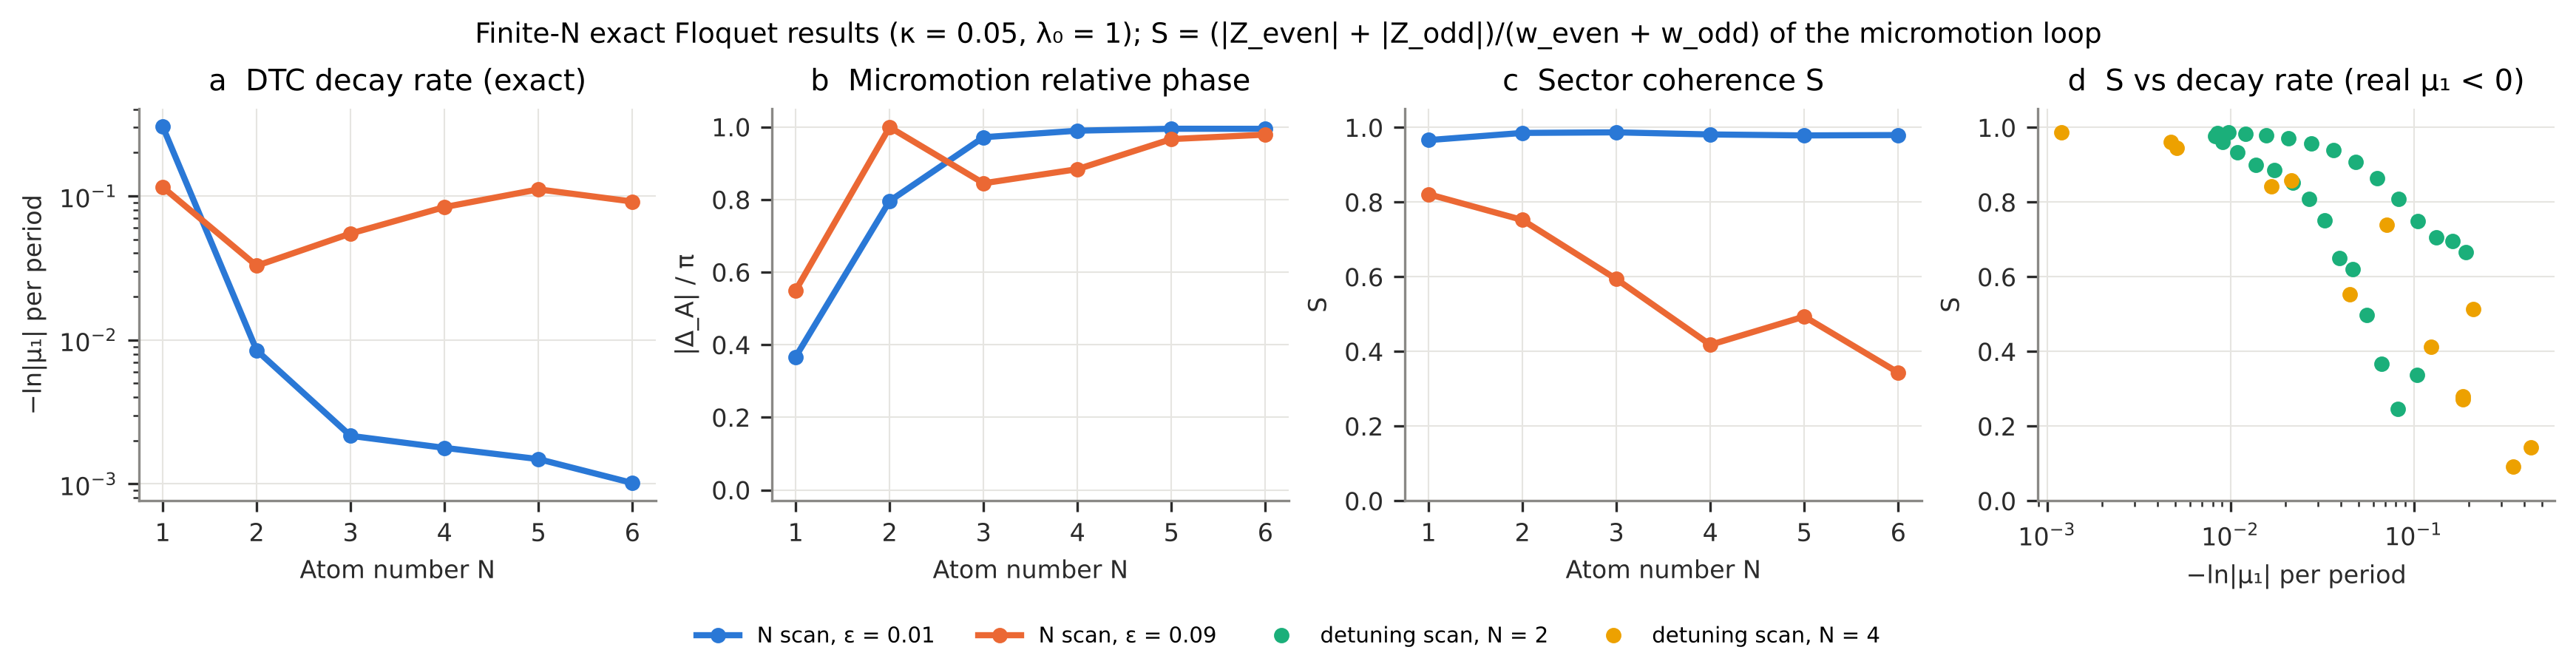
\includegraphics[width=\linewidth]{extension_finite_N.png}
\caption{Finite-$N$ exact Floquet results. (a)~Decay rate of the time-crystal mode against $N$:
monotonic in the pre-thermal regime ($\epsilon=0.01$), non-monotonic in the transient regime
($\epsilon=0.09$). (b)~Micromotion relative phase. (c)~Sector coherence $S$. (d)~$S$ against the
decay rate along the detuning scans.}
\label{fig:finite}
\end{figure}

%=========================================================================================
\section{Summary and outlook}\label{sec:summary}
%=========================================================================================

\begin{table}[h]
\centering
\small
\begin{tabular}{@{}p{4.3cm}p{5.0cm}p{5.6cm}@{}}
\toprule
Oscillator paper & Dicke / time-crystal counterpart & Result\\
\midrule
Generator $\hat n$, drive phase & $\Nex=\ad a+J_z+N/2$, counter-rotating phase $\theta$ & exact covariance \eqref{eq:covariance}; single-state formula \eqref{eq:loopB}\\
Weak drive: $\Gamma\propto E^2$ & normal phase: $\Gamma\propto\lambda^2$ & Eq.~\eqref{eq:weak} agrees to $0.1\%$ at weak coupling\\
Kerr DPTs & superradiant transition & $\Delta_B:0\to\pi$, sharpening with $N$; tracks the odd gap; visibility dip\\
Half loop with parity endpoint & period-doubled oscillator (lab frame) & quantized $\pi$ in the bright phase\\
--- & time crystal: loop A over one period & $e^{i\Delta_A}\to\operatorname{sgn}\mu_1$ (control experiment)\\
--- & finite-$N$ regimes & spectrum reproduces non-monotonic $N$; $S$ orders regimes along $\epsilon$, not along $N$\\
\bottomrule
\end{tabular}
\caption{How each ingredient of the oscillator paper carries over.}
\label{tab:summary}
\end{table}

\paragraph{The story in one paragraph.} Winding a drive phase produces a loop of steady states,
and its geometric phase diagnoses how the steady state is organized. For the open Dicke model the
natural drive phase is that of the counter-rotating coupling. Its loop is generated by the
excitation number and reduces exactly to a single-state formula. That GP reproduces the oscillator
paper's weak-drive physics, and it switches from $0$ to $\pi$ at the superradiant transition,
because a parity half-rotation exchanges the two symmetry-broken branches. A time crystal is more
than symmetry breaking: the \emph{drive} must exchange the branches every period. This is read by
the GP of the physical one-period loop of the Floquet steady state, which is quantized to $\pi$
when the branches are swapped and $0$ when they are not. The two-photon Kerr half loop of the
oscillator paper is the special case in which both loops coincide.

\paragraph{What is new and what is known.} That time crystals require $\mu_1\to-1$ is standard. In
\emph{closed} Floquet time crystals the $\pi$ splitting of parity partners has been reported to
be geometric in origin~\cite{schindler2024}. As far as we found (a limited search), the
open-system, mixed-state version is new:
\begin{itemize}
\item the exact covariance of the counter-rotating phase;
\item the quantized relative sector phase of the Floquet steady state, with its control
  experiment;
\item the reinterpretation of the Kerr half loop.
\end{itemize}

\paragraph{Limitations.}
\begin{itemize}
\item Exact numerics stop at $N\approx6$. A direct steady-state solve at $N=8$ ran over ten
  minutes and 3.6\,GB without finishing. The regime $N\sim20$–$500$ of Nguyen and Reichman needs
  an approximate two-branch description.
\item Only $\kappa=0.05$ was studied.
\item Loop A has no single-state reduction. It needs $\rho_F$ along the whole period, and its
  measurement is an open question.
\item For loop B, the Ramsey readout of~\cite{sun_gp} would need equal ancilla shifts from
  photons and atomic excitations; this has not been worked out.
\item The sum-level relative phase can be accidentally near $\pi$; pair-resolved quantities
  should be primary.
\end{itemize}

\paragraph{Next steps.}
\begin{enumerate}[label=(\arabic*)]
\item An analytic two-branch model for $\pi-\Delta$ in terms of branch overlap and tunnelling.
\item Larger $N$ through such a model, to reach the non-monotonic regime.
\item The paper's local response $\chi_\Gamma=\partial_x\arg Z$ and its split into $\chi_\lambda$
  and $\chi_n$ at the superradiant transition.
\item A measurement protocol for loop A.
\end{enumerate}

%=========================================================================================
\appendix
\section{Numerical methods and checks}\label{app:numerics}
%=========================================================================================

\begin{itemize}
\item \textbf{Floquet map.} $\E=e^{T_{\rm off}\Lio_{\rm off}}e^{T_{\rm on}\Lio_{\rm on}}$ is applied
  with sparse exponential actions, so no integration step crosses a switching time. Leading
  eigenvalues are obtained by Arnoldi iteration separately in the parity-even and parity-odd
  superoperator sectors. These agree with dense diagonalization of the map to $10^{-9}$.
\item \textbf{Steady states} of the undriven model are obtained by a sparse linear solve in the even
  sector with a trace constraint; slowest rates by shift-invert Arnoldi.
\item \textbf{Loop A.} $\rho_F$ is propagated on 400–800 steps per half period. Eigenvectors are
  followed by maximum-overlap assignment in each parity block, and the transport product is that of
  Eq.~\eqref{eq:tong}. The loop closes to $10^{-15}$, and step doubling changes $\Delta_A$ by
  $<5\times10^{-4}$\,rad. Eigenvectors with weight $<10^{-9}$ are not tracked; their total weight is
  reported.
\item \textbf{Loop B} uses the degeneracy-safe single-state formula, checked against the tracked
  orbit to $10^{-5}$.
\item \textbf{Convergence.} Fock cutoffs are chosen so that the top-three populations are
  $\le3\times10^{-5}$; selected points were repeated at larger cutoffs. The test suite (26 tests)
  covers the closed-form limits, including the exchanged-cat value $\pi[1-2N_B/\sinh2N_B]$ to five
  digits.
\item \textbf{Code and data.} \texttt{dicke\_floquet.py}, \texttt{dicke\_floquet\_scan.py},
  \texttt{dicke\_static\_scan.py}, \texttt{kerr\_parity\_half\_loop.py}; all numbers in this report
  are in \texttt{results/*.json}.
\end{itemize}

\begin{thebibliography}{99}\small
\bibitem{nguyen2026} H.~Nguyen and D.~R.~Reichman, \emph{Fate of discrete time crystals in finite-size cavity QED systems}, arXiv:2610.27589 (2026).
\bibitem{sun_gp} Z.~Sun, Y.~Shen, H.-T.~Ding, Y.~Zhan and L.-C.~Kwek, \emph{The geometric phase as a diagnostic for driven-dissipative oscillators}, manuscript and Supplementary Material.
\bibitem{gong2018} Z.~Gong, R.~Hamazaki and M.~Ueda, \emph{Discrete time-crystalline order in cavity and circuit QED systems}, Phys.\ Rev.\ Lett.\ \textbf{120}, 040404 (2018).
\bibitem{wilczek2012} F.~Wilczek, \emph{Quantum time crystals}, Phys.\ Rev.\ Lett.\ \textbf{109}, 160401 (2012).
\bibitem{bruno2013} P.~Bruno, \emph{Impossibility of spontaneously rotating time crystals: a no-go theorem}, Phys.\ Rev.\ Lett.\ \textbf{111}, 070402 (2013).
\bibitem{watanabe2015} H.~Watanabe and M.~Oshikawa, \emph{Absence of quantum time crystals}, Phys.\ Rev.\ Lett.\ \textbf{114}, 251603 (2015).
\bibitem{khemani2016} V.~Khemani, A.~Lazarides, R.~Moessner and S.~L.~Sondhi, \emph{Phase structure of driven quantum systems}, Phys.\ Rev.\ Lett.\ \textbf{116}, 250401 (2016).
\bibitem{else2016} D.~V.~Else, B.~Bauer and C.~Nayak, \emph{Floquet time crystals}, Phys.\ Rev.\ Lett.\ \textbf{117}, 090402 (2016).
\bibitem{sacha2018} K.~Sacha and J.~Zakrzewski, \emph{Time crystals: a review}, Rep.\ Prog.\ Phys.\ \textbf{81}, 016401 (2018).
\bibitem{zhang2017} J.~Zhang \emph{et al.}, \emph{Observation of a discrete time crystal}, Nature \textbf{543}, 217 (2017).
\bibitem{choi2017} S.~Choi \emph{et al.}, \emph{Observation of discrete time-crystalline order in a disordered dipolar many-body system}, Nature \textbf{543}, 221 (2017).
\bibitem{kessler2021} H.~Ke{\ss}ler \emph{et al.}, \emph{Observation of a dissipative time crystal}, Phys.\ Rev.\ Lett.\ \textbf{127}, 043602 (2021).
\bibitem{minganti2018} F.~Minganti, A.~Biella, N.~Bartolo and C.~Ciuti, \emph{Spectral theory of Liouvillians for dissipative phase transitions}, Phys.\ Rev.\ A \textbf{98}, 042118 (2018).
\bibitem{kirton2019} P.~Kirton, M.~M.~Roses, J.~Keeling and E.~G.~Dalla~Torre, \emph{Introduction to the Dicke model: from equilibrium to nonequilibrium, and vice versa}, Adv.\ Quantum Technol.\ \textbf{2}, 1800043 (2019).
\bibitem{tong2004} D.~M.~Tong, E.~Sj\"oqvist, L.~C.~Kwek and C.~H.~Oh, \emph{Kinematic approach to the mixed state geometric phase in nonunitary evolution}, Phys.\ Rev.\ Lett.\ \textbf{93}, 080405 (2004).
\bibitem{singh2003} K.~Singh, D.~M.~Tong, K.~Basu, J.~L.~Chen and J.~F.~Du, \emph{Geometric phases for nondegenerate and degenerate mixed states}, Phys.\ Rev.\ A \textbf{67}, 032106 (2003).
\bibitem{dimer2007} F.~Dimer, B.~Estienne, A.~S.~Parkins and H.~J.~Carmichael, \emph{Proposed realization of the Dicke-model quantum phase transition in an optical cavity QED system}, Phys.\ Rev.\ A \textbf{75}, 013804 (2007).
\bibitem{schindler2024} P.~M.~Schindler and M.~Bukov, \emph{Geometric Floquet theory}, arXiv:2410.07029 (2024).
\end{thebibliography}

\end{document}
